\section{Deep Learning\label{sec:DL}}
%%%%%%%%%%%%%%%%%%%%%%%%%%%%%%%%%%%%%%%%%%%%%%%%%%%%%%%%%%%%%%%%%%%%%%%%%%%%%%%%
\Gls{DL} is a field of \gls{ML} that is primarily concerned with the learning of
representations of data. At the core of \gls{DL} is the use of \glspl{MLP}, used
to model these representations. \Glspl{MLP} are fully connected layers of
biologically inspired artificial neurons, also known as \textbf{perceptrons}. A
brief history of these biologically inspired models is covered in
\autoref{ssec:perceptrons} with adapted notation from the field of \gls{DL}.
Although not all practices in \gls{DL}, strictly speaking, make use of
\glspl{MLP}, they are a fundamental concept which must be understood in the
stepping stones towards concepts of higher complexity in the field.
\autoref{ssec:mlps} covers this concept, extending directly on their composite
component: perceptrons.

\Glspl{MLP} are also called \textbf{feedfoward} as information is propagated in only a forward direction, as opposed to exhibiting \textbf{feedback} connections, where intermediate computations are fed back into the network. When feedforward networks are extended to include feedback connections, they are called \glspl{RNN}. These networks excel at learning temporal features, exhibiting a refined hypothesis space favouring sequenced information, such as a series of chronological observations. \autoref{ssec:rnn} covers this type of \gls{DNN}, and the prominent sub-type of \glspl{RNN}: \glspl{LSTM}.

\autoref{ssec:cnn} covers \gls{CNN}, a type of neural network similar to \glspl{MLP} and popular in contemporary research. These deep \glspl{NN} are essentially \glspl{MLP} which omit the property of being fully connected in favour of refining the hypothesis space towards detection of spatially-related features.

%The main difference between a \gls{NN} and a traditional \gls{ML} algorithm is
%that the neural network is a function of the data, rather than the data itself.

\subsection{Brief History of the Perceptron}\label{ssec:perceptrons}
%%%%%%%%%%%%%%%%%%%%%%%%%%%%%%%%%%%%%%%%%%%%%%%%%%%%%%%%%%%%%%%%%%%%%%%%%%%%%%%%

The McCullock-Pitts neuron, an earlier iteration of an artificial neuron, was
proposed by McCulloch and Pitts in the field of neuroscience in 1943
\cite{McCulloch1943}. Their work contended that neurons with a binary activation
function were analogous to first-order logic sentences. The perception of
artificial neurons changed with Hebb's work in 1949, where he proposed an idea
which has come to be known as Hebb's rule:

\begin{quote}
    Let us assume that the persistence or repetition of a reverberatory activity
    (or ``trace") tends to induce lasting cellular changes that add to its
    stability. [...] When an axon of cell A is near enough to excite a cell B
    and repeatedly or persistently takes part in firing it, some growth process
    or metabolic change takes place in one or both cells such that A’s
    efficiency, as one of the cells firing B, is increased. \cite{10.1007/978-3-642-70911-1_15}
\end{quote}

This theory is often summarised as \textit{``Cells that fires together, wire
together"} \cite{doi:10.1126/science.7912852}, which persists today in the
gradient-based learning at the core of contemporary \gls{DL}. The perceptron was
proposed by Rosenblatt \cite{Rosenblatt_1957_6098} in his technical report
funded by the United States Office of Naval Research
\cite{doi:10.1177/030631296026003005} in 1957. Rosenblatt incorporated Hebb's
findings into the McCullock-Pitts neuron.

The \textit{perceptron} is arguably the most fundamental concept in deep
learning, describing a mathematical model of a biological neuron. There are two
different sets of notation which exist when dealing with the bias of a
perceptron. One involves the inclusion of a unit constant in the input vector
$\mathbf{x}$, with the bias being specified by the value of the first weight
$w_0$. An alternative notation exists which treats the bias as a standalone
value $b$. The latter notation will be used, as it is the preferred notation in
contemporary deep learning research. The notation defining the mapping of a
perceptron is then: $f(\gls{ml:x};\glsvec{ml:w},
\gls{ml:b})=\gls{ml:x}^T\glsvec{ml:w}+\gls{ml:b}$;
$\gls{ml:x}\in\gls{set:R}[^{\gls{np:dim}[_\gls{fn:in}]}]$,
$\glsvec{ml:w}\in\gls{set:R}^{\gls{np:dim}[_\gls{fn:in}]}$, $\gls{ml:b}\in\gls{set:R}$. Furthermore
the model parameters, \glsvec{fn:param}, as introduced in
\autoref{sec:capoverunder}, are defined by the union of the bias and weight
vectors: $\glsvec{fn:param}=\{\glsvec{ml:w},\gls{ml:b}\}$.
\begin{figure}[htbp]
    \centering
    \input{graphics/tikz/perceptron_b}
    \captionsetup{format=hang} % hanging captions
    \caption{
        \textbf{Generalized illustration of a perceptron.} The mapping is
        defined by $f(\gls{ml:x};\glsvec{ml:w},
        \gls{ml:b})=\gls{ml:x}^T\glsvec{ml:w}+\gls{ml:b}$ where
        $\{\glsvec{ml:w},\gls{ml:b}\}=\glsvec{fn:param}$. The original formulation of
        the perceptron \cite{Rosenblatt_1957_6098} was intended to output a
        binary value, using a threshold step function, for classification
        purposes. The actual activation function \gls{dl:activation} has been
        generalized in order to relate the concept to modern deep learning
        techniques.
    }
    \label{fig:perceptron}
\end{figure}

\begin{equation}
    a=g\bigg(\sum_{k=0}^{\gls{np:dim}[_\gls{fn:in}]}{w_k}x_k + b\bigg)=g(z)
\end{equation}


%Rosenblatt's incorporated the model of  Rosenblatt
%incorporated the findings of Hebb \cite{10.1007/978-3-642-70911-1_15} into the
%model proposed by A set of inputs \gls{ml:x} would be weighted before being
%passed through a threshold step activation function \gls{dl:activation}.
%\autoref{fig:perceptron} shows a more general formulation which applies to the
%field of deep learning, with any activation function, \gls{dl:activation},
%mimicking a level of excitation akin to a biological neuron in response to its
%stimulus \gls{ml:x}.

\begin{figure}[!htp]
    \centering
    \begin{subfigure}[b]{0.70\textwidth}
        \centering
        \input{graphics/tikz/perceptron_and}
        \captionsetup{format=hang} % hanging captions
        \subcaption{Perceptron mapping}
        \label{fig:perceptron:and:mapping}
    \end{subfigure}\hfil
    \begin{subfigure}[b]{0.29\textwidth}
        \centering
        \renewcommand{\arraystretch}{1.5}
        \begin{tabular}{C{0.1\linewidth}C{0.1\linewidth}|C{0.1\linewidth}}
            \hline
            $x_1$ & $x_2$ & $y$ \\ \hline
            0     & 0     & 0   \\
            0     & 1     & 0   \\
            1     & 0     & 0   \\
            1     & 1     & 1
        \end{tabular}
        \vspace{0.5cm}
        \subcaption{Truth table}
        \label{fig:perceptron:and:truth}
    \end{subfigure}\hfil
    \captionsetup{format=hang} % hanging captions
    \caption{
        \textbf{Truth table of the AND logic gate.}
    }
    \label{fig:perceptron:and}
\end{figure}



Rosenblatt's statements caused an unfortunate controversy in the fledgling field
of \gls{AI}. According to the New York Times, he reported the perceptron to be
\textit{``the embryo of an electronic computer that [the Navy] expects will be
able to walk, talk, see, write, reproduce itself and be conscious of its
existence."} \cite{Olazaran1996} The backlash from the \gls{AI} community was
immense when results came nowhere close to this description, slowing progress
in the field overall.

\subsubsection{Perceptrons and Logic Gates}

In its original form, the perceptron was used as a supervised learning method
for binary classifiers. The primary criticism of the perceptron came in 1969
from Minsky and Papert \cite{minsky69perceptrons}, where it was shown that the
perceptron could only solve \textit{linearly separable} functions, and failed to
solve the XOR and NXOR functions. They claimed that the work being done in this
area was doomed to failure due to these limitations, resulting in little
subsequent research until about the 1980's.

%\newpage

\subsection{Multi-layer perceptrons}\label{ssec:mlps}
%%%%%%%%%%%%%%%%%%%%%%%%%%%%%%%%%%%%%%%%%%%%%%%%%%%%%%%%%%%%%%%%%%%%%%%%%%%%%%%%%
\textbf{Artificial neural networks} in the form of \Glspl{MLP}, or \textbf{feedforward neural networks}, are the fundamental models of \gls{DL}. These models are biologically inspired, and make direct use of the concept of the perceptron discussed in \autoref{ssec:perceptrons}. The primary extensions involve the use of a variety of activation functions other than the threshold step, and multiple layers of fully connected perceptrons often referred to as \textbf{neurons} or \textbf{units}. \Glspl{MLP} are characterized as being \textbf{fully-connected} which means that all the units in a layer are connected to all units in the next. These models are often referred to as \textbf{deep feedfoward networks} by virtue of having \textit{several} hidden layers. Note that there is no universally accepted definition of what integer values of perceptron layers \gls{dl:L} constitute deep and shallow networks, but generally speaking: a shallow network will usually have one hidden layer and a deep network will have several hidden layers. The mapping of an \gls{MLP} is defined by $\gls{y_pred}=f(\gls{ml:x}; \glsvec{fn:param})$; $\gls{ml:x}\in\gls{set:R}^{\gls{np:dim}[_\gls{fn:in}]}$; $\gls{y_pred}\in\gls{set:R}^{\gls{np:dim}[_\gls{fn:out}]}$.

\begin{figure}[htp]
    \centering
    % MIT License
%
% Copyright (c) 2021 Geoffrey H. Garrett
%
% Permission is hereby granted, free of charge, to any person obtaining a copy
% of this software and associated documentation files (the "Software"), to deal
% in the Software without restriction, including without limitation the rights
% to use, copy, modify, merge, publish, distribute, sublicense, and/or sell
% copies of the Software, and to permit persons to whom the Software is
% furnished to do so, subject to the following conditions:
%
% The above copyright notice and this permission notice shall be included in all
% copies or substantial portions of the Software.
%
% THE SOFTWARE IS PROVIDED "AS IS", WITHOUT WARRANTY OF ANY KIND, EXPRESS OR
% IMPLIED, INCLUDING BUT NOT LIMITED TO THE WARRANTIES OF MERCHANTABILITY,
% FITNESS FOR A PARTICULAR PURPOSE AND NONINFRINGEMENT. IN NO EVENT SHALL THE
% AUTHORS OR COPYRIGHT HOLDERS BE LIABLE FOR ANY CLAIM, DAMAGES OR OTHER
% LIABILITY, WHETHER IN AN ACTION OF CONTRACT, TORT OR OTHERWISE, ARISING FROM,
% OUT OF OR IN CONNECTION WITH THE SOFTWARE OR THE USE OR OTHER DEALINGS IN THE
% SOFTWARE.

%%%%%%%%%%%%%%%%%%%%%%%%%%%%%%%%%%%%%%%%%%%%%%%%%%%%%%%%%%%%%%%%%%%%%%%%%%%%%%%
% ACKNOWLEDGEMENTS
%%%%%%%%%%%%%%%%%%%%%%%%%%%%%%%%%%%%%%%%%%%%%%%%%%%%%%%%%%%%%%%%%%%%%%%%%%%%%%%
% Adapted from:
% https://www.researchgate.net/figure/The-agent-environment-interaction-in-reinforcement-learning_fig1_328494763

%%%%%%%%%%%%%%%%%%%%%%%%%%%%%%%%%%%%%%%%%%%%%%%%%%%%%%%%%%%%%%%%%%%%%%%%%%%%%%%
% DEPENDENCIES
%%%%%%%%%%%%%%%%%%%%%%%%%%%%%%%%%%%%%%%%%%%%%%%%%%%%%%%%%%%%%%%%%%%%%%%%%%%%%%%
%\usepackage{tikz}
%\usetikzlibrary{decorations.pathreplacing}    % for TikZ braces
%\usetikzlibrary{positioning}                  % for TikZ relative positioning

%%%%%%%%%%%%%%%%%%%%%%%%%%%%%%%%%%%%%%%%%%%%%%%%%%%%%%%%%%%%%%%%%%%%%%%%%%%%%%%
% USER STYLING
%%%%%%%%%%%%%%%%%%%%%%%%%%%%%%%%%%%%%%%%%%%%%%%%%%%%%%%%%%%%%%%%%%%%%%%%%%%%%%%

% TikZ node design.
\tikzset{basic/.style={draw,text width=1em,text badly centered}}
\tikzset{input/.style={basic, fill=green!25, circle}}
\tikzset{output/.style={basic, fill=blue!25, circle}}
\tikzset{weight/.style={basic,circle}}
\tikzset{hidden/.style={basic,circle}}
\tikzset{function/.style={basic,circle}}
\def\layersep{3em}
\def\transferx{9em}
\def\hiddenx{7em}
\def\hiddenxn{12em}


\def\sep{4em}
\def\L{\gls{L}}       % number of hidden layers
\def\y{\gls{y_true}}  % output vector
\def\x{\gls{ml:x}}    % input vector
\def\h{\gls{a_vec}}   % hidden output
\def\nx{\gls{ml:n_x}}   % hidden output
\def\ny{\gls{ml:n_y}}   % hidden output


%%%%%%%%%%%%%%%%%%%%%%%%%%%%%%%%%%%%%%%%%%%%%%%%%%%%%%%%%%%%%%%%%%%%%%%%%%%%%%%
% TIKZ PICTURE
%%%%%%%%%%%%%%%%%%%%%%%%%%%%%%%%%%%%%%%%%%%%%%%%%%%%%%%%%%%%%%%%%%%%%%%%%%%%%%%
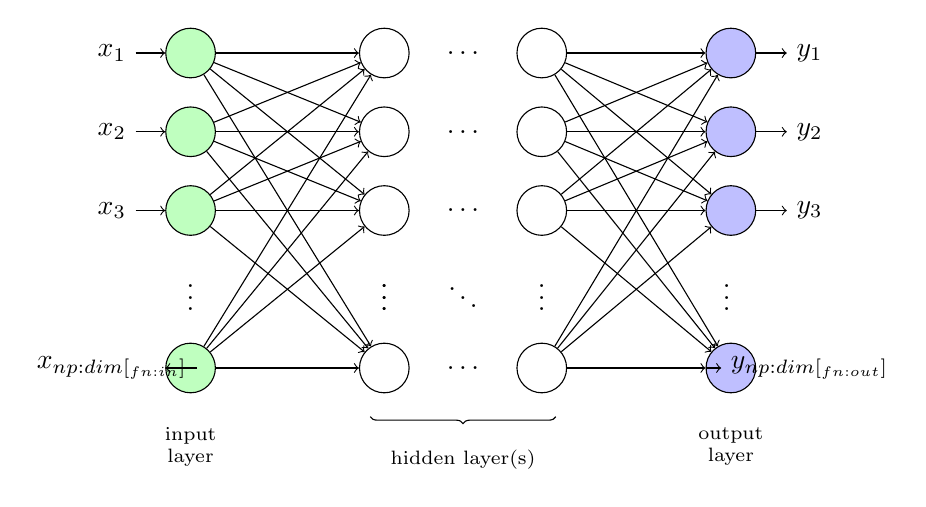
\begin{tikzpicture}
    \usetikzlibrary{decorations.pathreplacing}    % for TikZ braces
    \usetikzlibrary{positioning}                  % for TikZ relative positioning

    % input
    \foreach \n/\p in {0/1,1/2,2/3,3/4,4/5} {
        \ifnum \n=3
            % dots layer
            \node[] at (0, -\n) (X_\n) {$\vdots$};
            \node[] at (\hiddenx, -\n) (H1_\n) {$\vdots$};
            \node[right of=H1_\n] (M-\n) {$\ddots$};
            \node[below of=H1_2] (H2_\n) {$\vdots$};
            \node[below of=H2_2] (H2_\n) {$\vdots$};
            \node[right=5.7em of H2_\n] (Y_\n) {$\vdots$};
        \else
        \ifnum \n=4
            % n layer
            \node[input] at (0, -\n) (X_\n) {};
            \node[left of=X_\n] (I_\n) {$x_{\nx}$};
            \path[draw,->] (I_\n) -- (X_\n);
            \node[hidden] at (\hiddenx, -\n) (H1_\n) {}; %{$h_{n, 1}$};
            \node[right of= H1_\n] (M-\n) {$\ldots$};
            \node[hidden, right of= M-\n] (H2_\n) {}; % {$h_{n, m}$};
            \node[output, right= 5em of H2_\n] (Y_\n) {}; % {$h_{n, m}$};
            \node[right of=Y_\n] (O_\n) {$y_{\ny}$};
            \path[draw,->] (Y_\n) -- (O_\n);
        \else
            \node[input] at (0, -{\n}) (X_\n) {};
            \node[left of=X_\n] (I_\n) {$x_{\p}$};
            \path[draw,->] (I_\n) -- (X_\n);
            \node[hidden] at (\hiddenx, -\n) (H1_\n) {};%{$h_{\n, 1}$};
            \node[right of=H1_\n] (M-\n) {$\ldots$};
            \node[hidden, right of=M-\n] (H2_\n) {};% {$h_{\n, m}$};
            \node[output, right= 5em of H2_\n] (Y_\n) {}; % {$h_{n, m}$};
            \node[right of=Y_\n] (O_\n) {$y_\p$};
            \path[draw,->] (Y_\n) -- (O_\n);
        \fi
        \fi
    }

    % input layer connected to first hidden layer
    \foreach \j in {0,1,2,4} {
        \foreach \n in {0,1,2,4} {
            \path[draw,->] (X_\n) -- (H1_\j);
        }
    }

    % second hidden layer connected to output layer
    \foreach \j in {0,1,2,4} {
        \foreach \n in {0,1,2,4} {
            \path[draw,->] (H2_\n) -- (Y_\j);
        }
    }

    % labels
    \node[below of=X_4,font=\scriptsize, align=center] {input\\layer};
    \node[below of=Y_4,font=\scriptsize, align=center] {output\\layer};

    % brace for hidden layers
    \node[below=1em of M-4] (hidden-brace) {};
    \node[right=3em of hidden-brace] (hidden-brace-right) {};
    \node[left=3em of hidden-brace] (hidden-brace-left) {};
    \draw [decorate,decoration = {brace}] (hidden-brace-right) --  (hidden-brace-left);
    \node[below=0.5em of hidden-brace,font=\scriptsize] (hlayer) {hidden layer(s)};

\end{tikzpicture}


    \captionsetup{format=hang} % hanging captions
    \caption{
        \textbf{Generalized form of an \gls{MLP}}. Each layer, \textbf{excluding
        the input layer}, has associated weights, biases and activation
        functions. Furthermore, the layers are characterized as being
        \textbf{fully-connected}.
    }
    \label{fig:mlp}
\end{figure}

\autoref{fig:mlp} depicts the generalized concept of the \gls{MLP}. There are
three distinct types of layers: hidden, input, and output, for which
there is only one of each for the latter two. The input layer is simply the
input vector $\gls{ml:x}$, which does not have any weights, bias or activation
function associated to it.

\begin{figure}[htp]
    \centering
    % MIT License
%
% Copyright (c) 2021 Geoffrey H. Garrett
%
% Permission is hereby granted, free of charge, to any person obtaining a copy
% of this software and associated documentation files (the "Software"), to deal
% in the Software without restriction, including without limitation the rights
% to use, copy, modify, merge, publish, distribute, sublicense, and/or sell
% copies of the Software, and to permit persons to whom the Software is
% furnished to do so, subject to the following conditions:
%
% The above copyright notice and this permission notice shall be included in all
% copies or substantial portions of the Software.
%
% THE SOFTWARE IS PROVIDED "AS IS", WITHOUT WARRANTY OF ANY KIND, EXPRESS OR
% IMPLIED, INCLUDING BUT NOT LIMITED TO THE WARRANTIES OF MERCHANTABILITY,
% FITNESS FOR A PARTICULAR PURPOSE AND NONINFRINGEMENT. IN NO EVENT SHALL THE
% AUTHORS OR COPYRIGHT HOLDERS BE LIABLE FOR ANY CLAIM, DAMAGES OR OTHER
% LIABILITY, WHETHER IN AN ACTION OF CONTRACT, TORT OR OTHERWISE, ARISING FROM,
% OUT OF OR IN CONNECTION WITH THE SOFTWARE OR THE USE OR OTHER DEALINGS IN THE
% SOFTWARE.

%%%%%%%%%%%%%%%%%%%%%%%%%%%%%%%%%%%%%%%%%%%%%%%%%%%%%%%%%%%%%%%%%%%%%%%%%%%%%%%
% DEPENDENCIES
%%%%%%%%%%%%%%%%%%%%%%%%%%%%%%%%%%%%%%%%%%%%%%%%%%%%%%%%%%%%%%%%%%%%%%%%%%%%%%%
%\usepackage{tikz}
%\usetikzlibrary{decorations.pathreplacing}    % for TikZ braces
%\usetikzlibrary{positioning}                  % for TikZ relative positioning

%%%%%%%%%%%%%%%%%%%%%%%%%%%%%%%%%%%%%%%%%%%%%%%%%%%%%%%%%%%%%%%%%%%%%%%%%%%%%%%
% USER STYLING
%%%%%%%%%%%%%%%%%%%%%%%%%%%%%%%%%%%%%%%%%%%%%%%%%%%%%%%%%%%%%%%%%%%%%%%%%%%%%%%

% TikZ node design.
\tikzset{basic/.style={draw,text badly centered}}
\tikzset{input/.style={basic,minimum width=1.2cm, fill=green!25, circle}}
\tikzset{output/.style={basic,minimum width=1.2cm, fill=blue!25, circle}}
\tikzset{weight/.style={basic,circle}}
\tikzset{hidden/.style={basic,circle, minimum width=1.2cm}}
\tikzset{function/.style={basic,circle}}

\def\sep{4em}
\def\L{\gls{L}}       % number of hidden layers
\def\y{\gls{y_pred}}  % output vector
\def\x{\gls{ml:x}}    % input vector
\def\h{\gls{a_vec}}   % hidden output

%%%%%%%%%%%%%%%%%%%%%%%%%%%%%%%%%%%%%%%%%%%%%%%%%%%%%%%%%%%%%%%%%%%%%%%%%%%%%%%
% TIKZ PICTURE
%%%%%%%%%%%%%%%%%%%%%%%%%%%%%%%%%%%%%%%%%%%%%%%%%%%%%%%%%%%%%%%%%%%%%%%%%%%%%%%
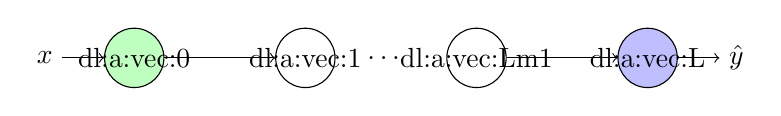
\begin{tikzpicture}
    \node[input, label={[xshift=-0.0em]center:\gls{dl:a:vec:0}}] (X) {\phantom{\gls{dl:a:vec:1}}};
    \node[, left=1.5em of X] (in) {$\bm{x}$};

    \node[hidden, right=\sep of X, label={[xshift=-0.0em]center:\gls{dl:a:vec:1}}] (H1) {\phantom{\gls{dl:a:vec:1}}};
    \node[hidden, right=\sep of H1, label={[xshift=-0.0em]center:\gls{dl:a:vec:Lm1}}] (H2) {\phantom{\gls{dl:a:vec:Lm1}}};
    \node[output, right=\sep of H2,  label={[xshift=-0.0em]center:\gls{dl:a:vec:L}}] (Y) {\phantom{\gls{dl:a:vec:L}}};
    \node[, right=1.5em of Y] (out) {$\bm{\hat{y}}$};

    \path[draw,->] (in) -- (X);
    \path[draw,->] (X) -- (H1);
    \node[right=0.8em of H1] (M) {$\ldots$};
    \path[draw,->] (H2) -- (Y);
    \path[draw,->] (Y) -- (out);
\end{tikzpicture}


    \captionsetup{format=hang} % hanging captions
    \caption{
        \textbf{Generalized vector form of an \gls{MLP}}. By notation, the
        input layer is denoted by $\gls{dl:a:vec:0}$ or $\gls{ml:x}$, the
        output layer is denoted by $\gls{dl:a:vec:L}$ or $\gls{y_pred}$, and the
        hidden layers as $\gls{dl:a:vec:l}\;\forall{}\;l\in\{1,...,\gls{dl:L}-1\}$.
    }
    \label{fig:mlp-vec}
\end{figure}

\autoref{fig:mlp} and \autoref{fig:mlp-vec} are equivalent and introduce the notation used for the variables of an artifical neural network. The vector form of the $l^\text{th}$ layer's activation variable is given by:

\begin{equation}
    \gls{dl:a:vec:l}
    = \gls{dl:g:l} \bigg(\gls{dl:w:l}^\text{T} \gls{dl:a:vec:lm1} + \gls{dl:b:l} \bigg)
    = \gls{dl:g:l}(\gls{dl:z:vec:l});
    \label{eq:mlp:a:vec}
\end{equation}

In the next section, where backpropagation is discussed, the following
scalar form of the activation will be used when deriving the expressions
used in the backpropagation algorithm:

\begin{equation}
    \gls{dl:a:l:j}
    = \gls{dl:g:l} \bigg(\sum_{k=0}^{{n_h}^{[l-1]}} \gls{dl:w:l:jk} \gls{dl:a:lm1:k} + \gls{dl:b:l:j} \bigg)
    = \gls{dl:g:l}(\gls{dl:z:l:j});
    \label{eq:mlp:a}
\end{equation}

Given an example of a network with two layers of perceptrons
($\gls{dl:L}=2$), the following set of equations (given by
\autoref{eq:mlp:a:vec}) define the \textbf{forward pass} or \textbf{forward
propagation} of information through the network:

\begin{equation}
    \begin{aligned}
        \gls{dl:a:vec:0} &= \gls{ml:x}; \\
        \gls{dl:a:vec:1} &= \gls{dl:g:1} \bigg(\gls{dl:W:1}^\text{T}\gls{dl:a:vec:0}  + \gls{dl:b:vec:1}\bigg); \\
        \gls{dl:a:vec:2} &= \gls{dl:g:2} \bigg(\gls{dl:W:2}^\text{T}\gls{dl:a:vec:1}  + \gls{dl:b:vec:2}\bigg) = \gls{y_pred}.
    \end{aligned}
\end{equation}

The number of model parameters $n_{\theta}$ for an \gls{MLP} can be calculated
as:

\begin{equation}
    n_{\theta}=\sum_{l=1}^{\gls{dl:L}} \gls{dl:nh:l} ({n_h}^{[l-1]} + 1)
\end{equation}


\newcommand\pardiff[2]{
    \frac{\partial{#1}}{\partial{#2}}
}

\subsection{Backpropagation}\label{ssec:backprop}

An important variable for the gradient-based optimization commonly used in neural architectures is the gradient of the cost function with respect to the model parameters $\nabla_{\gls{fn:param}}$\gls{dl:J}(\gls{fn:param}). This first-order partial differential is used to calculate updated estimates of the optimal set of model parameters \gls{fn:param}$^*$. Backpropagation is the technique used for this calculation. Using \autoref{eq:mlp:a}, we seek to find expressions for the first-order partial derivative of the cost function for the weights and biases of the network. Using the chain rule, we have:

\begin{equation}
    \pardiff{\gls{ml:J}}{\gls{dl:w:l:jk}} = \pardiff{\gls{ml:J}}{\gls{dl:z:l:j}}\pardiff{\gls{dl:z:l:j}}{\gls{dl:w:l:jk}}.
    \label{eq:bp:w:0}
\end{equation}

Following directly from  \autoref{eq:mlp:a}, the derivative of the $j^\text{th}$ unit's latent variable $z$ with respect to a weight associated to the unit $j$ in the previous layer is:

\begin{equation}
    \pardiff{\gls{dl:z:l:j}}{\gls{dl:w:l:jk}} = \gls{dl:a:lm1:k}.
    \label{eq:bp:w:1}
\end{equation}

Combining \autoref{eq:bp:w:0} and \autoref{eq:bp:w:1} gives:

\begin{equation}
    \pardiff{\gls{ml:J}}{\gls{dl:w:l:jk}} = \pardiff{\gls{ml:J}}{\gls{dl:z:l:j}}  \gls{dl:a:lm1:k}
    \label{eq:bp:w:2}
\end{equation}

A similar set of equations can be derived for the bias associated to the $j^\text{th}$ unit of a layer. Again, from the chain rule we have:

\begin{equation}
    \pardiff{\gls{ml:J}}{\gls{dl:b:l:j}} = \pardiff{\gls{ml:J}}{\gls{dl:z:l:j}}\pardiff{\gls{dl:z:l:j}}{\gls{dl:b:l:j}}.
    \label{eq:bp:b:0}
\end{equation}

The first order partial derivative of the latent variable $z$ with respect to the same unit's bias is:

\begin{equation}
    \pardiff{\gls{dl:z:l:j}}{\gls{dl:b:l:j}} = 1
    \label{eq:bp:b:1}
\end{equation}

Combining \autoref{eq:bp:b:0} and \autoref{eq:bp:b:1} gives:

\begin{equation}
    \pardiff{\gls{ml:J}}{\gls{dl:b:l:j}} = \pardiff{\gls{ml:J}}{\gls{dl:z:l:j}}.
    \label{eq:bp:b:2}
\end{equation}

The expression for $\partial\gls{ml:J}/\partial\gls{dl:z:l:j}$ depends on the architecture of the network in question, and unless it concerns the output layer, it will be comprised of numerous other partials from later layers in the network. For this reason, a table filling strategy sometimes called \textbf{dynamic programming}, is used \cite[p.~214]{Goodfellow-et-al-2016} to avoid redundant calculations (a.k.a. fancy bookkeeping).

\autoref{fig:mlp-example} shows the general way of illustrating an \gls{MLP} with 2 perceptron layers with 2 inputs, 2 hidden units and 2 outputs. It can be misleading to those unfamiliar with the simplifications made, following from the illustration of a perceptron in \autoref{ssec:perceptrons}. \autoref{fig:mlp-example-bp} shows the same network with all model parameters included for a concise illustration of the backpropagation algorithm.

\begin{figure}[htbp]
    \centering
    % MIT License
%
% Copyright (c) 2021 Geoffrey H. Garrett
%
% Permission is hereby granted, free of charge, to any person obtaining a copy
% of this software and associated documentation files (the "Software"), to deal
% in the Software without restriction, including without limitation the rights
% to use, copy, modify, merge, publish, distribute, sublicense, and/or sell
% copies of the Software, and to permit persons to whom the Software is
% furnished to do so, subject to the following conditions:
%
% The above copyright notice and this permission notice shall be included in all
% copies or substantial portions of the Software.
%
% THE SOFTWARE IS PROVIDED "AS IS", WITHOUT WARRANTY OF ANY KIND, EXPRESS OR
% IMPLIED, INCLUDING BUT NOT LIMITED TO THE WARRANTIES OF MERCHANTABILITY,
% FITNESS FOR A PARTICULAR PURPOSE AND NONINFRINGEMENT. IN NO EVENT SHALL THE
% AUTHORS OR COPYRIGHT HOLDERS BE LIABLE FOR ANY CLAIM, DAMAGES OR OTHER
% LIABILITY, WHETHER IN AN ACTION OF CONTRACT, TORT OR OTHERWISE, ARISING FROM,
% OUT OF OR IN CONNECTION WITH THE SOFTWARE OR THE USE OR OTHER DEALINGS IN THE
% SOFTWARE.

%%%%%%%%%%%%%%%%%%%%%%%%%%%%%%%%%%%%%%%%%%%%%%%%%%%%%%%%%%%%%%%%%%%%%%%%%%%%%%%
% ACKNOWLEDGEMENTS
%%%%%%%%%%%%%%%%%%%%%%%%%%%%%%%%%%%%%%%%%%%%%%%%%%%%%%%%%%%%%%%%%%%%%%%%%%%%%%%
% Design and implementation of this diagram was inspired and adapted from:
% https://tex.stackexchange.com/questions/104334/tikz-diagram-of-a-perceptron

%%%%%%%%%%%%%%%%%%%%%%%%%%%%%%%%%%%%%%%%%%%%%%%%%%%%%%%%%%%%%%%%%%%%%%%%%%%%%%%
% DEPENDENCIES
%%%%%%%%%%%%%%%%%%%%%%%%%%%%%%%%%%%%%%%%%%%%%%%%%%%%%%%%%%%%%%%%%%%%%%%%%%%%%%%
%\usepackage{tikz}
%\usetikzlibrary{decorations.pathreplacing}    % for TikZ braces
\usetikzlibrary{positioning}                  % for TikZ relative positioning

%%%%%%%%%%%%%%%%%%%%%%%%%%%%%%%%%%%%%%%%%%%%%%%%%%%%%%%%%%%%%%%%%%%%%%%%%%%%%%%
% USER STYLING
%%%%%%%%%%%%%%%%%%%%%%%%%%%%%%%%%%%%%%%%%%%%%%%%%%%%%%%%%%%%%%%%%%%%%%%%%%%%%%%

% TikZ node design.
\tikzset{basic/.style={draw,text width=1em,text badly centered}}
\tikzset{input/.style={basic, fill=green!25, circle}}
\tikzset{output/.style={basic, fill=blue!25, circle}}
\tikzset{weight/.style={basic,circle}}
\tikzset{hidden/.style={basic,circle}}
\tikzset{function/.style={basic,circle}}

\def\layersep{3.0em}
\def\layerseg{0.9em}
\def\transferx{9em}
\def\hiddenx{7em}
\def\hiddenxn{12em}

% Labels and symbols.
\def\activationlabel{threshold step}       % activation function label
\def\activationsymbol{$H$}                 % activation function symbol
\def\transferlabel{sum}                    % transfer function label
\def\transfersymbol{$\sum$}                   % transfer function symbol
\def\outputsymbol{$\text{OR}(x_1, x_2)$}   % output symbol
\def\inputsymbol{$x$}                      % input symbol
\def\inputvecsymbol{$\mathbf{x}$}          % input vector symbol
\def\weightslabel{weights}                 % input vector symbol
\def\biassymbol{$b$}                       % bias symbol

\def\sep{4em}
\def\L{\gls{L}}       % number of hidden layers
\def\y{\gls{y_true}}  % output vector
\def\x{\gls{ml:x}}    % input vector
\def\h{\gls{a_vec}}   % hidden output
\def\nx{\gls{np:dim}[_\gls{fn:in}]}   % hidden output
\def\ny{\gls{np:dim}[_\gls{fn:out}]}   % hidden output
\def\z{\gls{dl:z}}   % hidden output
\def\a{\gls{dl:a}}   % hidden output

%%%%%%%%%%%%%%%%%%%%%%%%%%%%%%%%%%%%%%%%%%%%%%%%%%%%%%%%%%%%%%%%%%%%%%%%%%%%%%%
% TIKZ PICTURE
%%%%%%%%%%%%%%%%%%%%%%%%%%%%%%%%%%%%%%%%%%%%%%%%%%%%%%%%%%%%%%%%%%%%%%%%%%%%%%%
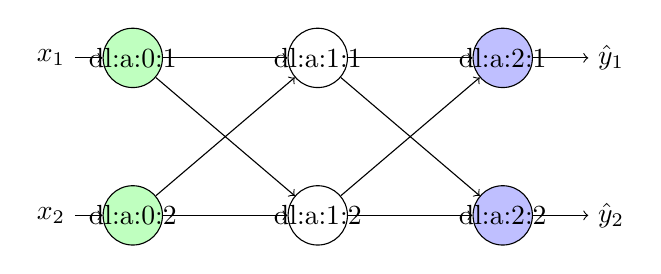
\begin{tikzpicture}

    \node[] at ({\transferx}, 0)                                                               (a1-center)   {};
    \node[left=\layersep of a1-center]                                                         (x-center)    {};

    \node[input, above of=x-center, label={[xshift=-0.0em]center:\gls{dl:a:0:1}}]              (a01)         {\phantom{\gls{dl:a:0:1}}};
    \node[input, below of=x-center, label={[xshift=-0.0em]center:\gls{dl:a:0:2}}]              (a02)         {\phantom{\gls{dl:a:0:2}}};

    \node[hidden, right=\layersep of a01, label={[xshift=-0.0em]center:\gls{dl:a:1:1}}]        (a11)         {\phantom{\gls{dl:a:1:1}}};
    \node[hidden, right=\layersep of a02, label={[xshift=-0.0em]center:\gls{dl:a:1:2}}]        (a12)         {\phantom{\gls{dl:a:1:2}}};

    \node[output, right=\layersep of a11, label={[xshift=-0.0em]center:\gls{dl:a:2:1}}]        (a21)         {\phantom{\gls{dl:a:2:1}}};
    \node[output, right=\layersep of a12, label={[xshift=-0.0em]center:\gls{dl:a:2:2}}]        (a22)         {\phantom{\gls{dl:a:2:2}}};

    \node[right=2em of a21]                                                                    (out1)         {$\hat{y}_1$};
    \node[right=2em of a22]                                                                    (out2)         {$\hat{y}_2$};
%

%    \node[input, below of=x-center] (a02) {};
    \node[, left=1em of a01]          (x-1) {$x_1$};
    \node[, left=1em of a02]          (x-2) {$x_2$};

    \path[draw,->] (x-1) -- (a01);
    \path[draw,->] (x-2) -- (a02);

    \path[draw,->] (a01) -- (a12);
    \path[draw,->] (a02) -- (a12);
%    \path[draw,->] (z12) -- (a12);

    \path[draw,->] (a01) -- (a11);
    \path[draw,->] (a02) -- (a11);
%    \path[draw,->] (z11) -- (a11);

    \path[draw,->] (a12) -- (a21);
    \path[draw,->] (a11) -- (a21);
    \path[draw,->] (a12) -- (a22);
    \path[draw,->] (a11) -- (a22);
%    \path[draw,->] (z21) -- (a21);

    \path[draw,->] (a21) -- (out1);
    \path[draw,->] (a22) -- (out2);


\end{tikzpicture}

    \captionsetup{format=hang} % hanging captions
    \caption{
        \textbf{Multi-layer perceptron mapping for an arbitrary network}
        with $\gls{dl:L}=2$ and $\{\gls{np:dim}[_\gls{fn:in}],n_h^{[1]},n_y\}=\{2,2,2\}$.
    }
    \label{fig:mlp-example}
\end{figure}
%\newpage
Deriving the expression for the partial of the cost function with respect to
$\gls{dl:w:1:22}$ and $\gls{dl:b:1:2}$ using \autoref{eq:bp:w:2} gives:

\begin{equation}
    \begin{aligned}
        \pardiff{\gls{ml:J}}{\gls{dl:w:1:22}}
        &=\pardiff{\gls{ml:J}}{\gls{dl:z:1:2}}\cdot{}\gls{dl:a:0:2};\\
        &=\pardiff{\gls{ml:J}}{\gls{dl:z:1:2}}\cdot{x_2};\\
        \pardiff{\gls{ml:J}}{\gls{dl:b:1:2}}
        &=\pardiff{\gls{ml:J}}{\gls{dl:z:1:2}}.
    \end{aligned}
\end{equation}


\begin{figure}[htbp]
    \centering
    % MIT License
%
% Copyright (c) 2021 Geoffrey H. Garrett
%
% Permission is hereby granted, free of charge, to any person obtaining a copy
% of this software and associated documentation files (the "Software"), to deal
% in the Software without restriction, including without limitation the rights
% to use, copy, modify, merge, publish, distribute, sublicense, and/or sell
% copies of the Software, and to permit persons to whom the Software is
% furnished to do so, subject to the following conditions:
%
% The above copyright notice and this permission notice shall be included in all
% copies or substantial portions of the Software.
%
% THE SOFTWARE IS PROVIDED "AS IS", WITHOUT WARRANTY OF ANY KIND, EXPRESS OR
% IMPLIED, INCLUDING BUT NOT LIMITED TO THE WARRANTIES OF MERCHANTABILITY,
% FITNESS FOR A PARTICULAR PURPOSE AND NONINFRINGEMENT. IN NO EVENT SHALL THE
% AUTHORS OR COPYRIGHT HOLDERS BE LIABLE FOR ANY CLAIM, DAMAGES OR OTHER
% LIABILITY, WHETHER IN AN ACTION OF CONTRACT, TORT OR OTHERWISE, ARISING FROM,
% OUT OF OR IN CONNECTION WITH THE SOFTWARE OR THE USE OR OTHER DEALINGS IN THE
% SOFTWARE.

%%%%%%%%%%%%%%%%%%%%%%%%%%%%%%%%%%%%%%%%%%%%%%%%%%%%%%%%%%%%%%%%%%%%%%%%%%%%%%%
% ACKNOWLEDGEMENTS
%%%%%%%%%%%%%%%%%%%%%%%%%%%%%%%%%%%%%%%%%%%%%%%%%%%%%%%%%%%%%%%%%%%%%%%%%%%%%%%
% Design and implementation of this diagram was inspired and adapted from:
% https://tex.stackexchange.com/questions/104334/tikz-diagram-of-a-perceptron

%%%%%%%%%%%%%%%%%%%%%%%%%%%%%%%%%%%%%%%%%%%%%%%%%%%%%%%%%%%%%%%%%%%%%%%%%%%%%%%
% DEPENDENCIES
%%%%%%%%%%%%%%%%%%%%%%%%%%%%%%%%%%%%%%%%%%%%%%%%%%%%%%%%%%%%%%%%%%%%%%%%%%%%%%%
%\usepackage{tikz}
%\usetikzlibrary{decorations.pathreplacing}    % for TikZ braces
\usetikzlibrary{positioning}                  % for TikZ relative positioning

%%%%%%%%%%%%%%%%%%%%%%%%%%%%%%%%%%%%%%%%%%%%%%%%%%%%%%%%%%%%%%%%%%%%%%%%%%%%%%%
% USER STYLING
%%%%%%%%%%%%%%%%%%%%%%%%%%%%%%%%%%%%%%%%%%%%%%%%%%%%%%%%%%%%%%%%%%%%%%%%%%%%%%%

% TikZ node design.
\tikzset{basic/.style={draw,text width=1em,text badly centered}}
\tikzset{input/.style={basic, fill=green!25, circle}}
\tikzset{output/.style={basic, fill=blue!25, circle}}
\tikzset{weight/.style={basic,circle}}
\tikzset{hidden/.style={basic,circle}}
\tikzset{function/.style={basic,circle}}

\def\layersep{4.5em}
\def\layerseg{0.9em}
\def\transferx{9em}
\def\hiddenx{7em}
\def\hiddenxn{12em}
\def\hh{2.5em}
\def\hv{3em}
\def\hvd{6em}
\def\zsep{6em}
\def\asep{4em}

% Labels and symbols.
\def\activationlabel{threshold step}       % activation function label
\def\activationsymbol{$H$}                 % activation function symbol
\def\transferlabel{sum}                    % transfer function label
\def\transfersymbol{$\sum$}                   % transfer function symbol
\def\outputsymbol{$\text{OR}(x_1, x_2)$}   % output symbol
\def\inputsymbol{$x$}                      % input symbol
\def\inputvecsymbol{$\mathbf{x}$}          % input vector symbol
\def\weightslabel{weights}                 % input vector symbol
\def\biassymbol{$b$}                       % bias symbol

\def\sep{4em}
\def\L{\gls{L}}       % number of hidden layers
\def\y{\gls{y_true}}  % output vector
\def\x{\gls{ml:x}}    % input vector
\def\h{\gls{a_vec}}   % hidden output
\def\nx{\gls{np:dim}[_\gls{fn:in}]}   % hidden output
\def\ny{\gls{np:dim}[_\gls{fn:out}]}   % hidden output
\def\z{\gls{dl:z}}   % hidden output
\def\a{\gls{dl:a}}   % hidden output

%%%%%%%%%%%%%%%%%%%%%%%%%%%%%%%%%%%%%%%%%%%%%%%%%%%%%%%%%%%%%%%%%%%%%%%%%%%%%%%
% TIKZ PICTURE
%%%%%%%%%%%%%%%%%%%%%%%%%%%%%%%%%%%%%%%%%%%%%%%%%%%%%%%%%%%%%%%%%%%%%%%%%%%%%%%
\begin{tikzpicture}

    \node[] at ({\transferx}, 0)                                                               (a0-center)   {};
    \node[input, above=\hv of a0-center, label={[xshift=-0.0em]center:\gls{dl:a:0:1}}]         (a01)         {\phantom{\gls{dl:a:0:1}}};
    \node[input, below=\hv of a0-center, label={[xshift=-0.0em]center:\gls{dl:a:0:2}}]         (a02)         {\phantom{\gls{dl:a:0:2}}};

    \node[, left=1em of a01]          (x-1) {$x_1$};
    \node[, left=1em of a02]          (x-2) {$x_2$};

    \node[right=\zsep of a0-center]                                                            (z1-center)   {};
    \node[hidden, above=\hv of z1-center, label={[xshift=-0.0em]center:\gls{dl:z:1:1}}]        (z11)         {\phantom{\gls{dl:z:1:1}}};
    \node[hidden, below=\hv of z1-center, label={[xshift=-0.0em]center:\gls{dl:z:1:2}}]        (z12)         {\phantom{\gls{dl:z:1:2}}};
    \node[, above of =z11, label={[xshift=-0.0em]center:\gls{dl:b:1:1}}]                       (b11)         {\phantom{\gls{dl:b:1:1}}};
    \node[, below of=z12, label={[xshift=-0.0em]center:\gls{dl:b:1:2}}]                        (b12)         {\phantom{\gls{dl:b:1:2}}};


    \node[right=\asep of z1-center]                                                            (a1-center)   {};
    \node[hidden, above=\hv of a1-center, label={[xshift=-0.0em]center:\gls{dl:a:1:1}}]        (a11)         {\phantom{\gls{dl:a:1:1}}};
    \node[hidden, below=\hv of a1-center, label={[xshift=-0.0em]center:\gls{dl:a:1:2}}]        (a12)         {\phantom{\gls{dl:a:1:2}}};

    \node[right=\zsep of a1-center]                                                            (z2-center)   {};
    \node[output, above=\hv of z2-center, label={[xshift=-0.0em]center:\gls{dl:z:2:1}}]        (z21)         {\phantom{\gls{dl:z:2:1}}};
    \node[output, below=\hv of z2-center, label={[xshift=-0.0em]center:\gls{dl:z:2:2}}]        (z22)         {\phantom{\gls{dl:z:2:2}}};
    \node[, above of =z21, label={[xshift=-0.0em]center:\gls{dl:b:2:1}}]                       (b21)         {\phantom{\gls{dl:b:2:1}}};
    \node[, below of=z22, label={[xshift=-0.0em]center:\gls{dl:b:2:2}}]                        (b22)         {\phantom{\gls{dl:b:2:2}}};

    \node[right=\asep of z2-center]                                                            (a2-center)   {};
    \node[output, above=\hv of a2-center, label={[xshift=-0.0em]center:\gls{dl:a:2:1}}]        (a21)         {\phantom{\gls{dl:a:2:1}}};
    \node[output, below=\hv of a2-center, label={[xshift=-0.0em]center:\gls{dl:a:2:2}}]        (a22)         {\phantom{\gls{dl:a:2:2}}};
    \node[right=2em of a21]                                                                    (out1)         {$\hat{y}_1$};
    \node[right=2em of a22]                                                                    (out2)         {$\hat{y}_2$};

    \path[draw,->] (x-1) -- (a01);
    \path[draw,->] (x-2) -- (a02);

    \path[draw,->] (a01) to [] node[above right, near end]{\gls{dl:w:1:12}}  (z12);
    \path[draw,->] (a02) to [] node[above, end]{\gls{dl:w:1:22}}  (z12);
    \path[draw,->] (b12) -- (z12);
    \path[draw,->] (z12) -- (a12);

    \path[draw,->] (a01) to [] node[above, end]{\gls{dl:w:1:11}}  (z11);
    \path[draw,->] (a02) to [] node[above left, near end]{\gls{dl:w:1:21}}  (z11);
    \path[draw,->] (b11) -- (z11);
    \path[draw,->] (z11) -- (a11);

    \path[draw,->] (a12) to [] node[above left, near end]{\gls{dl:w:2:21}}  (z21);
    \path[draw,->] (a12) to [] node[above, middle]{\gls{dl:w:2:22}}    (z22);
    \path[draw,->] (a11) to [] node[above, middle]{\gls{dl:w:2:11}}    (z21);
    \path[draw,->] (a11) to [] node[above right, near end]{\gls{dl:w:2:12}}  (z22);
    \path[draw,->] (z21) -- (a21);
    \path[draw,->] (b21) -- (z21);

    \path[draw,->] (z22) -- (a22);
    \path[draw,->] (b22) -- (z22);


    \path[draw,->] (a21) -- (out1);
    \path[draw,->] (a22) -- (out2);

    \def\bplinewidth{0.45mm}
    \path[draw, red, line width=\bplinewidth, dashed, ->]  (a12) -- (z12);
    \path[draw, red, line width=\bplinewidth, dashed, ->]  (z21) -- (a12);
    \path[draw, red, line width=\bplinewidth, dashed, ->]  (z22) -- (a12);
    \path[draw, red, line width=\bplinewidth, dashed, ->]  (a21) -- (z21);
    \path[draw, red, line width=\bplinewidth, dashed, ->]  (a22) -- (z22);


\end{tikzpicture}

    \captionsetup{format=hang} % hanging captions
    \caption{
        \textbf{Multi-layer perceptron mapping for an arbitrary network} with
        $\gls{dl:L}=2$ and $\{\gls{np:dim}[_\gls{fn:in}],n_h^{[1]},n_y\}=\{2,2,2\}$ expanded
        to show all model parameters and model variables. Emphasis has been
        placed on the backpropagation to determine the expression for
        $\partial\gls{ml:J}/\partial\gls{dl:z:1:2}$.
    }
    \label{fig:mlp-example-bp}
\end{figure}

The commonality between the updates of $\gls{dl:w:1:22}$ and $\gls{dl:b:1:2}$
are immediately clear, motivating the use of the previously mentioned table filling
strategy. The expression for $\partial\gls{ml:J}/\partial\gls{dl:z:1:2}$ can be determined
using the chain rule and following the influence of the output layer backwards
as seen in \autoref{fig:mlp-example-bp}, gives:

\begin{equation}
    \begin{aligned}
        \pardiff{\gls{ml:J}}{\gls{dl:z:1:2}}
        &= \pardiff{\gls{ml:J}}{\gls{dl:a:1:2}}\cdot{}\pardiff{\gls{dl:a:1:2}}{\gls{dl:z:1:2}}\\
        &= \bigg(\pardiff{\gls{ml:J}}{\gls{dl:z:2:1}}\cdot{}\pardiff{\gls{dl:z:2:1}}{\gls{dl:a:1:2}}
        +\pardiff{\gls{ml:J}}{\gls{dl:z:2:2}}\cdot{}\pardiff{\gls{dl:z:2:2}}{\gls{dl:a:1:2}}\bigg)
        \cdot{}g'^{\;[1]}(\gls{dl:z:1:2})\\
        &= \bigg(\pardiff{\gls{ml:J}}{\gls{dl:a:2:1}}\cdot{}g'^{\;[2]}(\gls{dl:z:2:1})\cdot{}\gls{dl:w:2:21}
        +\pardiff{\gls{ml:J}}{\gls{dl:a:2:2}}\cdot{}g'^{\;[2]}(\gls{dl:z:2:2})\cdot{}\gls{dl:w:2:22}\bigg)
        \cdot{}g'^{\;[1]}(\gls{dl:z:1:2})\\
        &= \bigg(\pardiff{\gls{ml:J}}{\hat{y}_1}\cdot{}g'^{\;[2]}(\gls{dl:z:2:1})\cdot{}\gls{dl:w:2:21}
        +\pardiff{\gls{ml:J}}{\hat{y}_2}\cdot{}g'^{\;[2]}(\gls{dl:z:2:2})\cdot{}\gls{dl:w:2:22}\bigg)
        \cdot{}g'^{\;[1]}(\gls{dl:z:1:2})
    \end{aligned}
    \label{eq:bp-deriv}
\end{equation}


%\begin{equation}
%    \frac{\partial{\gls{ml:J}}}{\partial{\gls{dl:theta:vec}}} = \bigg[
%        \frac{\partial{\gls{ml:J}}}{\partial{\gls{dl:theta:1}}},
%        \frac{\partial{\gls{ml:J}}}{\partial{\gls{dl:theta:2}}},
%        \ldots,
%        \frac{\partial{\gls{ml:J}}}{\partial{\gls{dl:theta:p}}}
%        \bigg]
%\end{equation}
%
%\begin{equation}
%    \begin{aligned}
%        \frac{\partial{\gls{ml:J}}}{\partial{\gls{dl:w:2:1}}}
%        =&
%        \frac{\partial{\gls{ml:J}}}{\partial{\gls{dl:a:2:1}}}
%        \frac{\partial{\gls{dl:a:2:1}}}{\partial{\gls{dl:w:2:1}}} \\
%        \frac{\partial{\gls{dl:a:2:1}}}{\partial{\gls{dl:w:2:1}}} \\
%        =&
%        \frac{\partial{\gls{ml:J}}}{\partial{\gls{dl:a:2:1}}}
%        \frac{\partial{\gls{dl:a:2:1}}}{\partial{\gls{dl:z:2:1}}}
%        \frac{\partial{\gls{dl:z:2:1}}}{\partial{\gls{dl:w:2:1}}} \\
%        =&
%        \frac{\partial{\gls{ml:J}}}{\partial{\gls{dl:a:2:1}}}
%        \frac{\partial{\gls{dl:a:2:1}}}{\partial{\gls{dl:z:2:1}}}
%        \frac{\partial{\gls{dl:z:2:1}}}{\partial{\gls{dl:w:2:1}}} \\
%        =&
%    \end{aligned}
%\end{equation}
%
%\begin{equation}
%    \frac{\partial{\gls{ml:J}}}{\partial{\gls{dl:w:2:2}}} =
%    \frac{\partial{\gls{ml:J}}}{\partial{\gls{dl:a:2:1}}}
%    \frac{\partial{\gls{dl:a:2:1}}}{\partial{\gls{dl:w:2:2}}}
%\end{equation}
%
%\begin{equation}
%    \frac{\partial{\gls{ml:J}}}{\partial{\gls{dl:b:2}}} =
%    \frac{\partial{\gls{ml:J}}}{\partial{\gls{dl:a:2:1}}}
%    \frac{\partial{\gls{dl:a:2:1}}}{\partial{\gls{dl:w:2:2}}}
%\end{equation}

\subsection{Activation function\label{activation_fn}}
%%%%%%%%%%%%%%%%%%%%%%%%%%%%%%%%%%%%%%%%%%%%%%%%%%%%%%%%%%%%%%%%%%%%%%%%%%%%%%%%

The trend of activation functions in neural networks is that more and more non-saturated activation functions are being used to improve the performance of deep neural networks. The main benefit of using these activation functions is that they can help to avoid the so-called vanishing gradient problem, which can impede the convergence speed of a neural network.

There are several different types of activation functions that can be used in deep neural networks. Some of the most common ones include those that follow in this section.

\subsubsection{Sigmoid}\label{ssec:sigmoid}
    
The sigmoid function is a saturated activation function that has been used for many years, but it has been shown to have some limitations in terms of its performance. Some key points to take away from the sigmoid activation function include the following:

\begin{itemize}
    \item The sigmoid function is a continuous function, which means that it is differentiable everywhere.
    \item The derivatives of the sigmoid function are easily calculated.
    \item The sigmoid function was commonly used in shallow neural networks.
    \item In addition, the sigmoid function is frequently employed in the output level of a neural network owing to its value distribution.
    \item While the sigmoid function is rarely adopted in deep neural networks except for the output level, it suffers from the limitations of soft saturation.
\end{itemize}

\subsubsection{Hyperbolic Tangent (TanH)}\label{ssec:hyperbolic_tangent}

The hyperbolic tangent is an example of another saturated activation function that has been used in deep neural networks, but similarly to the sigmoid, it has also been shown to have some limitations in terms of its performance. Some key points to take away from the hyperbolic tangent activation function include the following:

\begin{itemize}
    \item The hyperbolic tangent function is continuous and monotonic, and it is differentiable everywhere.
    \item It is symmetric about the origin, of which the outputs, namely the inputs of the next layer, are more likely on average close to zero.
    \item Neural networks with hyperbolic tangent activation functions converge faster than those with sigmoid activation functions.
    \item Furthermore, neural networks with hyperbolic tangent activation functions have lower classification errors than those with sigmoid activation functions,
    \item therefore, the hyperbolic tangent is generally preferred over the use of sigmoid activation functions.
    \item A disadvantage is that the calculation of the derivatives of hyperbolic tangent functions is more complicated than the sigmoid function. 
    \item It has the same soft saturation as the sigmoid function, which also has the vanishing gradient problem.
\end{itemize}

In conclusion, neural networks with hyperbolic tangent activation functions can learn faster than those with sigmoid activation functions. This is because hyperbolic tangent activation functions are more efficient and produce sparse outputs, which is hypothesised as being due to this behaviour more closely resembling the actual operating mode of cortical neurons.

\subsubsection{Rectified Linear Unit (ReLU)}\label{ssec:rectified_linear_unit}

The \gls{RELU} is a non-saturated activation function that is very effective in avoiding the vanishing gradient problem \cite{Hara2015}. Some key advantages of the \gls{RELU} activation function over the sigmoid and hyperbolic tangent activation functions include the following:

\begin{itemize}
    \item Reduced computational cost compared to sigmoid and hyperbolic tangent functions.
    \item Faster convergence than saturating activation functions \cite{Hara2015}.
    \item Easier sparsity in the activations of neuron units. One advantage of the \gls{RELU} activation function is that it allows a network to easily obtain sparse representation. More specifically, the output is 0 when the input x<0, which provides the sparsity in the activation of neuron units and improves the efficiency of data learning. When the input x≥0, the features of the data can be retained largely \cite{Hara2015}.
    \item Derivatives can be set as constant, improving convergence speed. This avoids being trapped in a local optimum and resolves the vanishing gradient effect that occurred in sigmoid and hyperbolic tangent activation functions \cite{Fahlman1988}.
    \item Can reach the best performance without unsupervised pre-training \cite{pmlr-v15-glorot11a}.
\end{itemize}

\subsubsection{Leaky Rectified Linear Unit (LReLU)}\label{ssec:leaky_relu}

\gls{LRELU} is a variant of the \gls{RELU} activation function which aims at addressing the tendency of ``dead (or dying) \gls{RELU}'' neurons occurring as a result of the zero gradients in the negative part of the \gls{RELU} function which halts learning in that region of its domain \cite{Hara2015}. The key points of \gls{LRELU} and other augmented variants are:

\begin{itemize}
    \item The \gls{LRELU} activation function is a modification of the \gls{RELU} activation function that allows for small negative values when the input is less than zero.
    \item This allows for a small, non-zero gradient when the unit is saturated and not active, which can help improve the learning process \cite{Maas2013}.
    \item The PreLU and \gls{RRELU} activation functions are also modifications of the \gls{RELU} function that can help improve learning by preventing vanishing gradients.
\end{itemize}

\subsubsection{Exponetial Linear Unit (ELU)}

The \gls{ELU} is another non-saturated activation function, and it is even more effective than \gls{RELU} in avoiding the vanishing gradient problem.

\begin{itemize}
    \item \gls{ELU} has a left-saturation which allows deep neural networks to be more robust to input perturbations or noise.
    \item The output average of \gls{ELU} is close to zero, which contributes to faster convergence.
    \item Experimental results have shown that \gls{ELU} can enable faster learning and improved generalization performance, partly due to the output average of an \gls{ELU} approaching zero.
    \item It has an additional parameter (often denoted as $\alpha$) which manages the value to which an \gls{ELU} saturates for negative network inputs \cite{Maas2013}.
\end{itemize}

\subsubsection{Swish}\label{ssec:swish}

Swish is a smooth, non-monotonic activation function that outperforms ReLU on deep networks applied to a variety of challenging domains, developed by Google. 

\begin{itemize}
    \item Its simplicity and similarity to \gls{RELU} means that \glspl{RELU} can be replaced with Swish units in any neural network with ease.
    \item Its performance in comparison to ReLU, suggests that even when varying the batch size, it outperforms ReLU.
    \item Swish consistently matches or outperforms ReLU in deep neural network applications in challenging domains (i.e. image classification and machine translation) \cite{Ramachandran2017}.
    \item Deeper Swish networks can be trained than ReLU variants. This is because Swish has a gradient squishing property, which helps to prevent over-fitting and results in more accurate models. 
\end{itemize}

\subsubsection{Sinusoidal representation network (SIREN)}\label{ssec:siren}

\gls{SIREN} offers several potential benefits over conventional continuous and discrete representations \cite{Sitzmann2020}, including:

\begin{itemize}
    \item Accurate representations of natural signals, such as images, audio, and video in a deep learning framework.
    \item Derivatives and Laplacians of the target signal are implicitly learned when the network is trained on the target signal.
    \item A single \gls{SIREN} can be trained on the target signal, its derivative, and its Laplacian simultaneously.
    \item Constrained and unconstrained boundary value problems can be solved robustly using \gls{SIREN}. 
\end{itemize}

A key success with \glspl{SIREN} is the promising results shown by Izzo et al. \cite{IzzoGeodesyNet2021, IzzoBennu2021} when applied to the modelling of irregularly shaped small bodies with heterogeneous mass distribution, for the reconstruction of the gravitational potential field with and without provided body shapes.


% The choice of activation functions in deep networks has a significant effect on
% the training dynamics and task performance. Currently, the most successful and
% widely-used activation function is the Rectified Linear Unit (ReLU). Although
% various hand-designed alternatives to ReLU have been proposed, none have managed to replace it due to inconsistent gains. In this work, we propose to leverage automatic search techniques to discover new activation functions. Using
% a combination of exhaustive and reinforcement learning-based search, we discover multiple novel activation functions. We verify the effectiveness of the
% searches by conducting an empirical evaluation with the best discovered activation function. Our experiments show that the best discovered activation function,
% f(x) = x · sigmoid(βx), which we name Swish, tends to work better than ReLU
% on deeper models across a number of challenging datasets. For example, simply
% replacing ReLUs with Swish units improves top-1 classification accuracy on ImageNet by 0.9% for Mobile NASNet-A and 0.6% for Inception-ResNet-v2. The
% simplicity of Swish and its similarity to ReLU make it easy for practitioners to
% replace ReLUs with Swish units in any neural network.

% A wide variety of activation functions $\phi$ have been used and improved upon
% the threshold step function. The primary concept used in motivating different
% activation functions is the problem of \textbf{vanishing gradient} when using
% deep neural networks. A vanishing gradient is a phenomenon that occurs in deep
% neural networks when calculating the partial derivative of the cost function
% associated with the weights being updated. \autoref{eq:bp-deriv} shows that when
% the gradient of a unit in a layer (e.g. $g'^{\;[2]}$), becomes small
% (learning is nearly complete), the backpropagated gradients to earlier weights
% (e.g. $\gls{dl:w:2:22}$) become increasingly small. This phenomenon is worsened
% by activation functions whose gradients are zero in regions of their input
% domain, effectively halting learning.

% The Sigmoid function (a.k.a. the logistic function) was introduced to replace
% the step function in the initial design of the perceptron
% (\autoref{ssec:perceptrons}), which has no gradients to be exploited by gradient
% descent methods. The sigmoid exhibits problems with vanishing gradients due to
% the saturation that occurs at 0 and 1 in the output, where gradients are
% extremely close to zero. In addition to vanishing gradients, the derivative is
% computationally expensive when networks become large. A similar activation
% function to the Sigmoid is the hyperbolic tangent (TanH) function, seen in
% \autoref{}. Tanh suffers from the same problems as the Sigmoid. The main
% difference between the two is that the output of TanH is zero-centred in the
% range of -1 to 1, which has been known to improve convergence in learning
% \autoref{}. The problems faced by the Sigmoid and TanH functions motivated a
% simpler activation: the ReLU (\autoref{}), which has become the most commonly
% used in the field of \gls{DL}.

% The sigmoid function (seen in \autoref{}) has been one of the most widely
% used activation functions in machine learning

%\begin{figure}[htbp]
%    \centering
%    \makeatletter
\pgfmathdeclarefunction{erf}{1}{%
    \begingroup
    \pgfmathparse{#1 > 0 ? 1 : -1}%
    \edef\sign{\pgfmathresult}%
    \pgfmathparse{abs(#1)}%
    \edef\x{\pgfmathresult}%
    \pgfmathparse{1/(1+0.3275911*\x)}%
    \edef\t{\pgfmathresult}%
    \pgfmathparse{%
        1 - (((((1.061405429*\t -1.453152027)*\t) + 1.421413741)*\t
        -0.284496736)*\t + 0.254829592)*\t*exp(-(\x*\x))}%
    \edef\y{\pgfmathresult}%
    \pgfmathparse{(\sign)*\y}%
    \pgfmath@smuggleone\pgfmathresult%
    \endgroup
}
%dep
%subfig
\begin{figure}[t!]
    \centering
    \subfloat[Threshold Step]{
        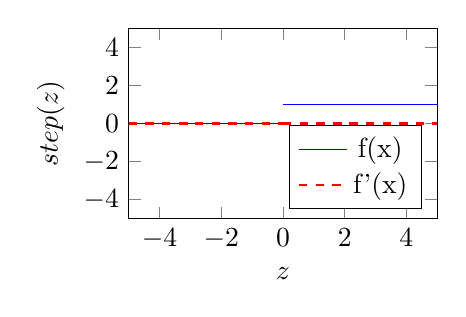
\begin{tikzpicture}
            \begin{axis}
                [width=5.5cm,height=4cm,ylabel=$step(z)$,xlabel=$z$,ymin=-5.0,ymax=5.0,xmin=-5,xmax=5,
                legend style={at={(0.95,0.05)},anchor=south east},]
                \addplot[blue,smooth, domain=-5:0] {0};
                \addplot[red,dashed, thick, domain=-5:0] {0};
                \addplot[blue,smooth, domain=-0:5] {1};
                \addplot[red,dashed, thick, domain=-0:5] {0};
                \addlegendentry{f(x)}
                \addlegendentry{f'(x)}
            \end{axis}
        \end{tikzpicture}
    }
    \subfloat[Linear]{
        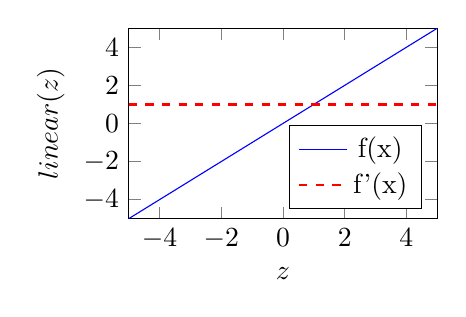
\begin{tikzpicture}
            \begin{axis}
                [width=5.5cm,height=4cm,ylabel=$linear(z)$,xlabel=$z$,ymin=-5.0,ymax=5.0,xmin=-5,xmax=5,
                legend style={at={(0.95,0.05)},anchor=south east},]
                \addplot[blue,smooth] {x};
                \addlegendentry{f(x)}
                \addplot[red,dashed, thick] {1};
                \addlegendentry{f'(x)}
            \end{axis}
        \end{tikzpicture}
    }
    \subfloat[Sigmoid]{
        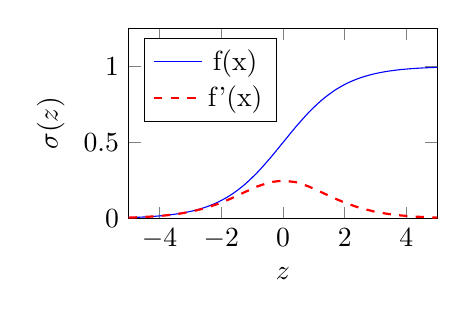
\begin{tikzpicture}
            \begin{axis}
                [width=5.5cm,height=4cm,ylabel=$\sigma(z)$,xlabel=$z$,ymin=0,ymax=1.25,xmin=-5,xmax=5,
                legend style={at={(0.05,0.95)},anchor=north west},]
                \addplot[blue,smooth] {1/(1+exp(-x))};
                \addlegendentry{f(x)}
                \addplot[red, dashed, thick] {1/(1+exp(-x)) * (1-1/(1+exp(-x)))};
                \addlegendentry{f'(x)}
            \end{axis}
        \end{tikzpicture}
    }\\
    \subfloat[Hyperbolic tangent]{
        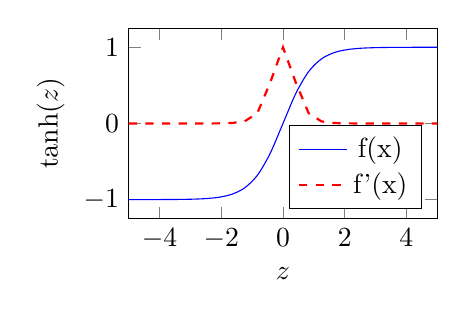
\begin{tikzpicture}
            \begin{axis}
                [width=5.5cm,height=4cm,ylabel=$\tanh(z)$,xlabel=$z$,ymin=-1.25,ymax=1.25,xmin=-5,xmax=5, legend style={at={(0.95,0.05)},anchor=south east},]
                \addplot[blue,smooth] {tanh(x)};
                \addlegendentry{f(x)}
                \addplot[red,dashed, thick] {1/cosh(2*x)*1/cosh(2*x)};
                \addlegendentry{f'(x)}
            \end{axis}
        \end{tikzpicture}
    }
    \subfloat[ReLU]{
        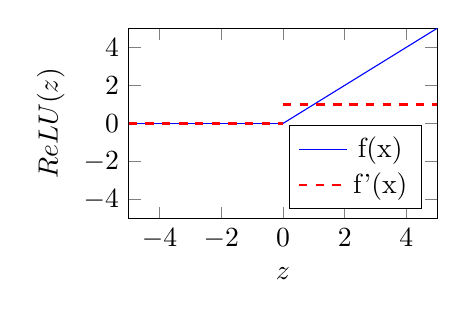
\begin{tikzpicture}
            \begin{axis}
                [width=5.5cm,height=4cm,ylabel=$ReLU(z)$,xlabel=$z$,ymin=-5.0,ymax=5.0,xmin=-5,xmax=5,
                legend style={at={(0.95,0.05)},anchor=south east},]
                \addplot[blue,smooth, domain=-5:0] {0};
                \addplot[red,dashed, thick, domain=-5:0] {0};
                \addplot[blue,smooth, domain=-0:5] {x};
                \addplot[red,dashed, thick, domain=-0:5] {1};
                \addlegendentry{f(x)}
                \addlegendentry{f'(x)}
            \end{axis}
        \end{tikzpicture}
    }
    \subfloat[Leaky ReLU]{
        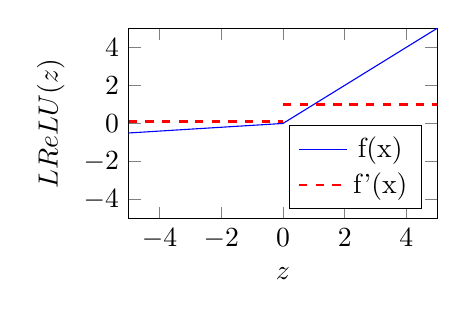
\begin{tikzpicture}
            \begin{axis}
                [width=5.5cm,height=4cm,ylabel=$LReLU(z)$,xlabel=$z$,ymin=-5.0,ymax=5.0,xmin=-5,xmax=5,
                legend style={at={(0.95,0.05)},anchor=south east},]
                \addplot[blue,smooth, domain=-5:0] {0.1*x};
                \addplot[red,dashed, thick, domain=-5:0] {0.1};
                \addplot[blue,smooth, domain=-0:5] {x};
                \addplot[red,dashed, thick, domain=-0:5] {1};
                \addlegendentry{f(x)}
                \addlegendentry{f'(x)}
            \end{axis}
        \end{tikzpicture}
    }\\
    \subfloat[GELU]{
        \begin{tikzpicture}
            \begin{axis}
                [width=5.5cm,height=4cm,ylabel=$GELU(z)$,xlabel=$z$,ymin=-5.0,ymax=5.0,xmin=-5,xmax=5,
                legend style={at={(0.95,0.05)},anchor=south east},]
                \addplot[blue,smooth] {x * 0.5 * (1 + erf(x /sqrt(2)))};
                \addplot[red,dashed, thick] {0.5 * (1 + erf(x /sqrt(2))) + 1/sqrt(2*pi) * (exp(-x*x/2))};
                \addlegendentry{f(x)}
                \addlegendentry{f'(x)}
            \end{axis}
        \end{tikzpicture}
    }
    \subfloat[Swish]{
        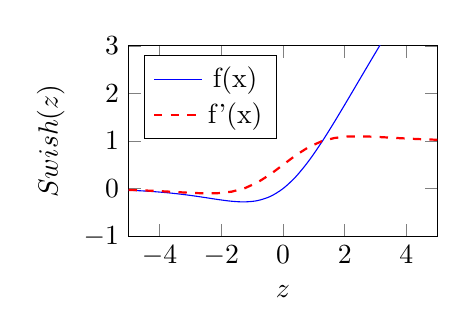
\begin{tikzpicture}
            \begin{axis}
                [width=5.5cm,height=4cm,ylabel=$Swish(z)$,xlabel=$z$,ymin=-1,ymax=3.0,xmin=-5,xmax=5,
                legend style={at={(0.05,0.95)},anchor=north west},]
                \addplot[blue,smooth] {x*(1/(1+exp(-x)))}; % f (x) + σ (x) (1 − f (x))
                \addlegendentry{f(x)}
                \addplot[red, dashed, thick] {x/(1+exp(-x)) + 1/(1+exp(-x)) * (1-x/(1+exp(-x)))};
                \addlegendentry{f'(x)}
            \end{axis}
        \end{tikzpicture}
    }
    \subfloat[]{
        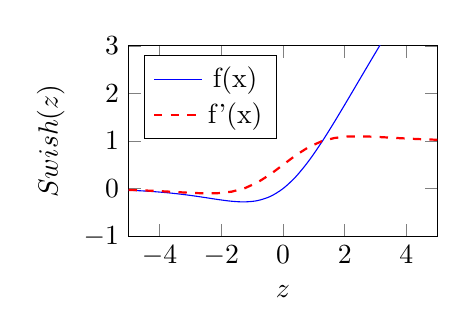
\begin{tikzpicture}
            \begin{axis}
                [width=5.5cm,height=4cm,ylabel=$Swish(z)$,xlabel=$z$,ymin=-1,ymax=3.0,xmin=-5,xmax=5,
                legend style={at={(0.05,0.95)},anchor=north west},]
                \addplot[blue,smooth] {x*(1/(1+exp(-x)))}; % f (x) + σ (x) (1 − f (x))
                \addlegendentry{f(x)}
                \addplot[red, dashed, thick] {x/(1+exp(-x)) + 1/(1+exp(-x)) * (1-x/(1+exp(-x)))};
                \addlegendentry{f'(x)}
            \end{axis}
        \end{tikzpicture}
    }
    \caption[Sigmoidal activation functions.]{Commonly used activation functions in MLPs.}
    \label{fig:activation-functions}
\end{figure}
%    \caption{Activation functions}
%    \label{fig:activation}
%\end{figure}
\vspace{2em}
\makeatletter
\pgfmathdeclarefunction{erf}{1}{%
    \begingroup
    \pgfmathparse{#1 > 0 ? 1 : -1}%
    \edef\sign{\pgfmathresult}%
    \pgfmathparse{abs(#1)}%
    \edef\x{\pgfmathresult}%
    \pgfmathparse{1/(1+0.3275911*\x)}%
    \edef\t{\pgfmathresult}%
    \pgfmathparse{%
        1 - (((((1.061405429*\t -1.453152027)*\t) + 1.421413741)*\t
        -0.284496736)*\t + 0.254829592)*\t*exp(-(\x*\x))}%
    \edef\y{\pgfmathresult}%
    \pgfmathparse{(\sign)*\y}%
    \pgfmath@smuggleone\pgfmathresult%
    \endgroup
}
%dep
%subfig
\begin{figure}[t!]
    \centering
    \subfloat[Threshold Step]{
        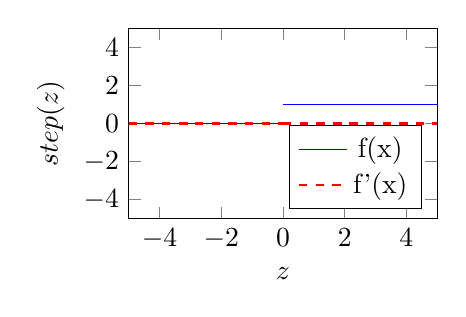
\begin{tikzpicture}
            \begin{axis}
                [width=5.5cm,height=4cm,ylabel=$step(z)$,xlabel=$z$,ymin=-5.0,ymax=5.0,xmin=-5,xmax=5,
                legend style={at={(0.95,0.05)},anchor=south east},]
                \addplot[blue,smooth, domain=-5:0] {0};
                \addplot[red,dashed, thick, domain=-5:0] {0};
                \addplot[blue,smooth, domain=-0:5] {1};
                \addplot[red,dashed, thick, domain=-0:5] {0};
                \addlegendentry{f(x)}
                \addlegendentry{f'(x)}
            \end{axis}
        \end{tikzpicture}
    }
    \subfloat[Linear]{
        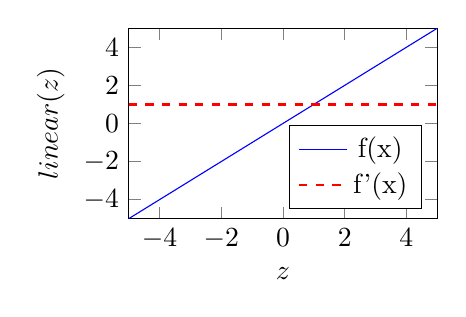
\begin{tikzpicture}
            \begin{axis}
                [width=5.5cm,height=4cm,ylabel=$linear(z)$,xlabel=$z$,ymin=-5.0,ymax=5.0,xmin=-5,xmax=5,
                legend style={at={(0.95,0.05)},anchor=south east},]
                \addplot[blue,smooth] {x};
                \addlegendentry{f(x)}
                \addplot[red,dashed, thick] {1};
                \addlegendentry{f'(x)}
            \end{axis}
        \end{tikzpicture}
    }
    \subfloat[Sigmoid]{
        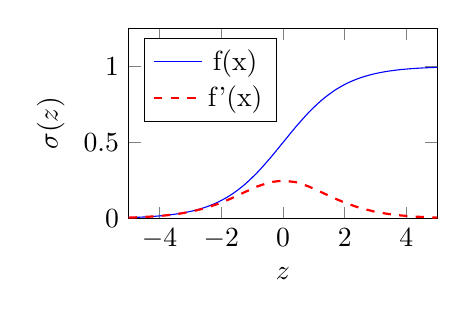
\begin{tikzpicture}
            \begin{axis}
                [width=5.5cm,height=4cm,ylabel=$\sigma(z)$,xlabel=$z$,ymin=0,ymax=1.25,xmin=-5,xmax=5,
                legend style={at={(0.05,0.95)},anchor=north west},]
                \addplot[blue,smooth] {1/(1+exp(-x))};
                \addlegendentry{f(x)}
                \addplot[red, dashed, thick] {1/(1+exp(-x)) * (1-1/(1+exp(-x)))};
                \addlegendentry{f'(x)}
            \end{axis}
        \end{tikzpicture}
    }\\
    \subfloat[Hyperbolic tangent]{
        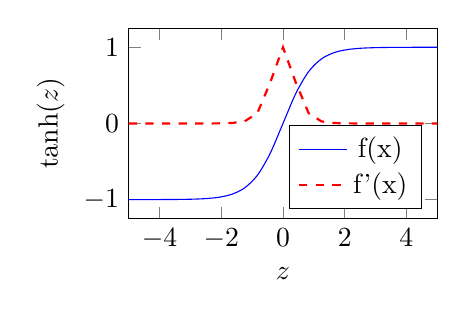
\begin{tikzpicture}
            \begin{axis}
                [width=5.5cm,height=4cm,ylabel=$\tanh(z)$,xlabel=$z$,ymin=-1.25,ymax=1.25,xmin=-5,xmax=5, legend style={at={(0.95,0.05)},anchor=south east},]
                \addplot[blue,smooth] {tanh(x)};
                \addlegendentry{f(x)}
                \addplot[red,dashed, thick] {1/cosh(2*x)*1/cosh(2*x)};
                \addlegendentry{f'(x)}
            \end{axis}
        \end{tikzpicture}
    }
    \subfloat[ReLU]{
        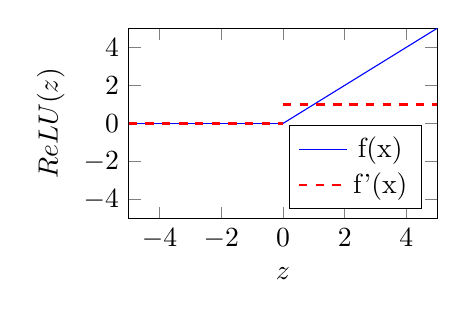
\begin{tikzpicture}
            \begin{axis}
                [width=5.5cm,height=4cm,ylabel=$ReLU(z)$,xlabel=$z$,ymin=-5.0,ymax=5.0,xmin=-5,xmax=5,
                legend style={at={(0.95,0.05)},anchor=south east},]
                \addplot[blue,smooth, domain=-5:0] {0};
                \addplot[red,dashed, thick, domain=-5:0] {0};
                \addplot[blue,smooth, domain=-0:5] {x};
                \addplot[red,dashed, thick, domain=-0:5] {1};
                \addlegendentry{f(x)}
                \addlegendentry{f'(x)}
            \end{axis}
        \end{tikzpicture}
    }
    \subfloat[Leaky ReLU]{
        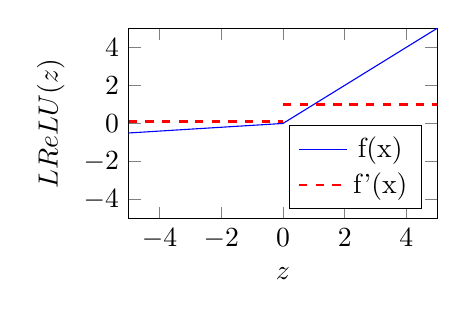
\begin{tikzpicture}
            \begin{axis}
                [width=5.5cm,height=4cm,ylabel=$LReLU(z)$,xlabel=$z$,ymin=-5.0,ymax=5.0,xmin=-5,xmax=5,
                legend style={at={(0.95,0.05)},anchor=south east},]
                \addplot[blue,smooth, domain=-5:0] {0.1*x};
                \addplot[red,dashed, thick, domain=-5:0] {0.1};
                \addplot[blue,smooth, domain=-0:5] {x};
                \addplot[red,dashed, thick, domain=-0:5] {1};
                \addlegendentry{f(x)}
                \addlegendentry{f'(x)}
            \end{axis}
        \end{tikzpicture}
    }\\
    \subfloat[GELU]{
        \begin{tikzpicture}
            \begin{axis}
                [width=5.5cm,height=4cm,ylabel=$GELU(z)$,xlabel=$z$,ymin=-5.0,ymax=5.0,xmin=-5,xmax=5,
                legend style={at={(0.95,0.05)},anchor=south east},]
                \addplot[blue,smooth] {x * 0.5 * (1 + erf(x /sqrt(2)))};
                \addplot[red,dashed, thick] {0.5 * (1 + erf(x /sqrt(2))) + 1/sqrt(2*pi) * (exp(-x*x/2))};
                \addlegendentry{f(x)}
                \addlegendentry{f'(x)}
            \end{axis}
        \end{tikzpicture}
    }
    \subfloat[Swish]{
        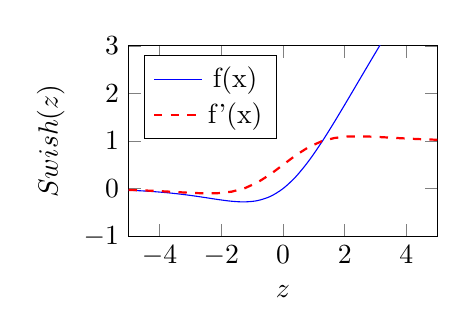
\begin{tikzpicture}
            \begin{axis}
                [width=5.5cm,height=4cm,ylabel=$Swish(z)$,xlabel=$z$,ymin=-1,ymax=3.0,xmin=-5,xmax=5,
                legend style={at={(0.05,0.95)},anchor=north west},]
                \addplot[blue,smooth] {x*(1/(1+exp(-x)))}; % f (x) + σ (x) (1 − f (x))
                \addlegendentry{f(x)}
                \addplot[red, dashed, thick] {x/(1+exp(-x)) + 1/(1+exp(-x)) * (1-x/(1+exp(-x)))};
                \addlegendentry{f'(x)}
            \end{axis}
        \end{tikzpicture}
    }
    \subfloat[]{
        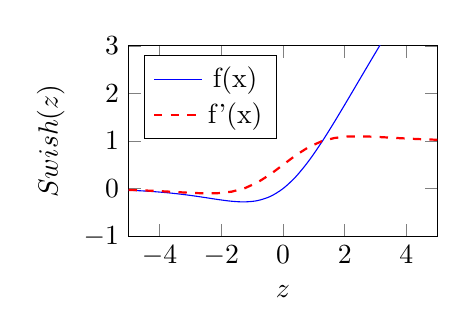
\begin{tikzpicture}
            \begin{axis}
                [width=5.5cm,height=4cm,ylabel=$Swish(z)$,xlabel=$z$,ymin=-1,ymax=3.0,xmin=-5,xmax=5,
                legend style={at={(0.05,0.95)},anchor=north west},]
                \addplot[blue,smooth] {x*(1/(1+exp(-x)))}; % f (x) + σ (x) (1 − f (x))
                \addlegendentry{f(x)}
                \addplot[red, dashed, thick] {x/(1+exp(-x)) + 1/(1+exp(-x)) * (1-x/(1+exp(-x)))};
                \addlegendentry{f'(x)}
            \end{axis}
        \end{tikzpicture}
    }
    \caption[Sigmoidal activation functions.]{Commonly used activation functions in MLPs.}
    \label{fig:activation-functions}
\end{figure}
% \textcolor{red}{(Caption needs further elaboration, and the bottom right graph must be removed)}
%
\subsection{Optimisation of Artificial Neural Networks}\label{dl:optimisation}
%%%%%%%%%%%%%%%%%%%%%%%%%%%%%%%%%%%%%%%%%%%%%%%%%%%%%%%%%%%%%%%%%%%%%%%%%%%%%%%%

It was seen in \autoref{ssec:backprop} that the partial differential of \gls{ml:J} can be expressed as a function of the model parameters of an \gls{MLP}. These first-order expressions can therefore be used in gradient optimisation of the network. This is referred to as \textbf{gradient descent}, of which there are three variants which differ in their use of the training dataset.

\begin{itemize}
    \item \textbf{\Gls{GD}}, a.k.a. batch gradient descent or vanilla gradient
    descent computes the gradient of the cost function over the entire training
    dataset and performs a single update:
    \begin{equation}
        \gls{dl:theta}_{t+1} = \gls{dl:theta}_t - \gls{dl:lr} \nabla_{\gls{dl:theta}}\gls{dl:J}(\gls{dl:theta}_t)
        \label{eq:dl:opt:gd}
    \end{equation}
    This method of gradient descent can be slow and intractable for datasets
    that do not fit in memory. This method of optimization is also incompatible
    with \textit{online} learning. \cite{ruder2017overview}

    \item \textbf{\Gls{SGD}} computes the gradient of the cost function for
    \textit{each} example in the dataset and performs an update for each
    input-output pair in the dataset:
    \begin{equation}
        \gls{dl:theta}_{t+1} = \gls{dl:theta}_t - \gls{dl:lr} \nabla_{\gls{dl:theta}}\gls{dl:J}(\gls{dl:theta}_t;\glsvec{fn:in}^{\gls{ml:ith:xy}},\glsvec{fn:out}^{\gls{ml:ith:xy}})
        \label{eq:dl:opt:sgd}
    \end{equation}
    Batch gradient descent often results in redundant gradient calculations for
    large datasets when encountering similar examples. \Gls{SGD} overcomes this
    redundancy, however, it exhibits updates with high variance which can cause
    high fluctuations in the cost function. These high fluctuations result in
    overshooting of the minima being converged towards, and therefore often
    requires a lower learning rate than \Gls{GD}. \cite{ruder2017overview}

    \item \textbf{\Gls{MB-SGD}} has the advantages of both \gls{SGD} and \gls{GD},
    computing the gradient of the cost function for every mini-batch of \gls{ml:m}
    training examples:
    \begin{equation}
        \gls{dl:theta}_{t+1} = \gls{dl:theta}_t - \gls{dl:lr} \nabla_{\gls{dl:theta}}\gls{dl:J}(\gls{dl:theta}_t;\gls{ml:x:i:i+m},\gls{ml:y_true:i:i+m})
        \label{eq:dl:opt:mb_sgd}
    \end{equation}
    Memory constraints are no longer encountered (as in \Gls{GD}), and high
    variance in updates are avoided (as in \Gls{SGD}). Mini-batch gradient
    descent methods are the typical choice when training a neural architecture
    \cite{ruder2017overview}. \textbf{Note} that the term \Gls{SGD} is very
    often used in literature to refer to \Gls{MB-SGD}.

\end{itemize}

Some challenges exist for vanilla gradient descent methods, most of which
concern the topology of the cost function. Constant learning rates can lead to
slow convergence, especially when a saddle point is encountered in the cost
function in non-convex problems, which are notoriously difficult to escape. This
motivates the need to schedule, adapt or augment the learning rate throughout
the learning process. These issues are addressed by the specific variants of the
optimization algorithms used. For the next section, the parameters in the
notation $\nabla_{\gls{dl:theta}}\gls{dl:J}(\gls{dl:theta}_k; \ldots)$ are
dropped, as it is implicitly defined by the choice of batch size in \Gls{MB-SGD}
(as mentioned, a.k.a. \gls{SGD}).

\begin{figure}[htp]
    %%%%%%%%%%%%%%%%%%%%%%%%%%%%%%%%%%%%%%%%%%%%%%%%%%%%%%%%%%%%%%%%%%%%%%%%%%%%%%%%%%%
    \begin{subfigure}[b]{0.49\textwidth}
        \centering
        \begin{tikzpicture}
    \begin{axis}
        [samples=20,
        ylabel=$\theta_2$,
        xlabel=$\theta_1$,
        zlabel=$\gls{ml:J}(\gls{dl:theta})$,
        ticks=none,
        xticklabels={\empty},
        yticklabels={\empty},
        ]
        \addplot3[
        surf,
        domain y=0:15,
        domain=-3.141:3.141,
        ] {-125*(cos(deg(x)))+y^2};
        \addplot3[color=black,mark=o] table[col sep=comma] {code/output/vanilla_lr0.015.csv};
    \end{axis}
\end{tikzpicture}
        \subcaption{Slow learning rate (Low $\gls{dl:lr}$)}
        \label{fig:gd-low-eta}
    \end{subfigure}\hfil
    %%%%%%%%%%%%%%%%%%%%%%%%%%%%%%%%%%%%%%%%%%%%%%%%%%%%%%%%%%%%%%%%%%%%%%%%%%%
    \begin{subfigure}[b]{0.49\textwidth}
        \centering
        \input{graphics/tikz/vanilla_gd_med_eta}
        \subcaption{Medium learning rate (Medium $\gls{dl:lr}$)}
        \label{fig:gd-medium-eta}
    \end{subfigure}\hfil
    %%%%%%%%%%%%%%%%%%%%%%%%%%%%%%%%%%%%%%%%%%%%%%%%%%%%%%%%%%%%%%%%%%%%%%%%%%%%%%%%%%%
    \captionsetup{format=hang} % hanging captions
    \caption{
        An illustration of \gls{SGD} at varied levels of learning rate
        (\gls{dl:lr}), in the convergence of the cost function optimization
        (\gls{ml:J}) with a ravine-like topology. \gls{SGD} notoriously has
        trouble navigating ravines, seen by its oscillation across the slops of
        the ravine, with hesitant progress towards the minima. a) shows a very
        slow convergence with a constant low setting of $\gls{dl:lr}$. b) shows
        an overshooting of the ravine's trough with a constant medium setting of
        \gls{dl:lr}. There exists a third case where \gls{dl:lr} is set to an
        excessive value, causing the first update to exit the ravine-like
        topology entirely.
    }
    \label{fig:vanilla-gd-learning}
\end{figure}

\subsubsection{Gradient descent optimization algorithms}
%\hline

\textbf{Momentum}~\cite{QIAN1999145} was introduced to deal with the problem
that \gls{SGD} exhibits in ravine-like topology
(\autoref{fig:vanilla-gd-learning}), accelerating the descent along the relevant
direction, while dampening it in the other direction~\cite{ruder2017overview}.
This technique is often compared to that of a ball rolling down a ravine, with
momentum building up in the relevant direction.
This is achieved through adding a fraction ($\gamma$) of the previous update to
the current update:
\begin{equation}
    \begin{aligned}
        \bm{v}_t                  &= \gamma{}\bm{v}_{t-1} + \gls{dl:lr} \nabla_{\gls{dl:theta}}\gls{dl:J}(\gls{dl:theta}_t) \\
        \gls{dl:theta}_{t+1} &= \gls{dl:theta}_t - \bm{v}_t
        \label{eq:dl:opt:sgd_momentum}
    \end{aligned}
\end{equation}

\textbf{\Gls{NAG}}~\cite{Nesterov1983AMF} addresses a shortcoming of momentum.
This technique adds a mechanism which can be compared to a \textit{smarter} ball
rolling down the hill, which slows down before the hill slopes up again after
the lowest point. This is achieved through the use of the momentum term $\gamma
\bm{v}_{t-1}$, although the gradient of cost function is evaluated at
$\gls{dl:theta}_t-\gamma \bm{v}_{t-1}$, a rough guess where the parameters are going
to be, rather than $\gls{dl:theta}_t$:
\begin{equation}
    \begin{aligned}
        \bm{v}_t &= \gamma \bm{v}_{t-1} + \gls{dl:lr} \nabla_{\gls{dl:theta}}\gls{dl:J}(\gls{dl:theta}_k - \gamma \bm{v}_{t-1}) \\
        \gls{dl:theta}_{t+1} &= \gls{dl:theta}_t - \bm{v}_t
    \end{aligned}
\end{equation}

\textbf{Adagrad} \cite{JMLR:v12:duchi11a} adapts the learning rate
according to the historical updates of the parameters. Larger updates are
carried out for infrequently updated parameters, and smaller for those more
frequently updated. This property makes this algorithm perform well for sparsely
distributed data. The following is often set for simplicity in literature:
\begin{equation}
    g_{t,i} = \nabla_{\gls{dl:theta}_i} \gls{dl:J}(\gls{dl:theta}_k)
\end{equation}
Adagrad modifies the learning rate $\eta$ at each time step $t$ using the
past computed gradients for each parameter $\theta_i$ as:
\begin{equation}
    \gls{dl:theta}_{t+1,i} = \gls{dl:theta}_{t,i} -\frac{\gls{dl:lr}}{\sqrt{G_{t,ii}+\epsilon}}\cdot{g_{t,i}}
\end{equation}
Where $G_t$ is a diagonal matrix where each element $i,i$ corresponds to the sum
of the squares of all historical gradients of $g_i$, expressed by:
\begin{equation}
    G_t = \sum_{t=1}^T \bm{g}_{\tau}^2
\end{equation}
A smoothing factor $\epsilon$ is used to avoid division by zero, typically set
as $1e-8$. The primary benefit of Adagrad is the elimination of the need to
manually tune $\gls{dl:lr}$, it is typically set and left at
$0.01$~\cite{ruder2017overview}. The primary weakness of Adagrad is that the
accumulated sum of squares of the gradient continuously grows during training,
causing the learning rate to asymptotically approach zero.

\textbf{Adadelta}~\cite{zeiler2012adadelta} is an extension of Adagrad
which aims to reduce its aggressive, monotomically decreasing learning rate.
Adadelta achieves this by storing a running average of the squared gradient
updates within a window, defined by a fraction $\gamma$ (similar to that seen in
momentum):
\begin{equation}
    \gls{E} [g^2]_t = \gamma{}\gls{E} [g^2]_{t-1} + (1-\gamma) g_t^2
\end{equation}
The fraction $\gamma$ is typically set at $0.9$ giving an effective window width
of 10 for the running average. The original authors introduce a second exponentially
decaying average, the running average of the squared gradient updates:
\begin{equation}
    \gls{E} [\Delta{\theta}^2]_t = \gamma{}\gls{E} [\Delta{\theta}^2]_{t-1} +
    (1-\gamma)\Delta{\theta}^2_{t}
\end{equation}
From these expectations, the author approximates the RMS of the gradients and
parameter updates as:
\begin{equation}
    \begin{aligned}
        \text{RMS}[g]              & = \sqrt{\gls{E} [g^2] + \epsilon} \\
        \text{RMS}[\Delta{\theta}] & = \sqrt{\gls{E} [\Delta{\theta}^2] + \epsilon}, \\
    \end{aligned}
\end{equation}
from which the final expression for the parameter updates is expressed:
\begin{equation}
    \begin{aligned}
        \Delta{\gls{dl:theta}_t} &= - \frac{\text{RMS}[\Delta{\gls{dl:theta}}]_{t-1}}{\text{RMS}[\bm{g}]_t}\cdot{}\bm{g}_t \\
        \gls{dl:theta}_{t+1} &= \gls{dl:theta}_t + \Delta{\gls{dl:theta}_t}
    \end{aligned}
\end{equation}
The motivation and derivation of the implementation are omitted here but can be
found in literature \cite{zeiler2012adadelta, ruder2017overview}. The key
takeaway is that there is no need to set the learning rate $\gls{dl:lr}$ to a
fixed value.

\textbf{RMSProp}, or root mean square propagation, is a method used to optimize Artificial Neural Networks (ANNs). RMSProp is a learning method that has been growing in popularity among scientists and researchers. It extends the Stochastic Gradient Descent algorithm, as well as the momentum method. Additionally, it forms the foundation of the Adam algorithm \cite{ruder2017overview, JMLR:v12:duchi11a}. The RMSProp derivation is similar to that of Adadelta:

\begin{equation}
    \begin{aligned}
        \gls{E} [\Delta{\theta}^2] &= \gamma{}\gls{E} [\Delta{\theta}^2]_{t-1} + (1-\gamma)\Delta{\theta}^2_{t} \\
        \gls{dl:theta}_{t+1}       &= \gls{dl:theta}_t + \frac{\gls{dl:lr}}{\sqrt{\gls{E} [\Delta{\theta}^2]_t+\epsilon}}\bm{g}_t
    \end{aligned}
\end{equation}

An commonly suggested balue for $\gamma$ is $0.9$, and \gls{dl:lr} is often set to $0.001$.

\textbf{Adam} is a popular, adaptive gradient descent optimization algorithm that has been shown to work well in practice. It maintains a per-parameter learning rate that is adapted based on the average of recent magnitudes of the gradients, which makes it suitable for online and non-stationary problems. It is also computationally efficient and has few memory requirements. It is a combination of the advantages of RMSProp and momentum. The Adam algorithm is expressed as follows:

\begin{equation}
    \begin{aligned}
        m_t &= \beta_1 m_{t-1} + (1-\beta_1)\bm{g}_t \\
        v_t &= \beta_2 v_{t-1} + (1-\beta_2)\bm{g}_t^2, \\
    \end{aligned}
\end{equation}

where $m_t$ and $v_t$ are estimates of the first moment and the second moment of the gradients respectively. The bias-corrected first and second-moment estimates are given by:

\begin{equation}
    \begin{aligned}
        \hat{m}_t &= \frac{m_t}{1-\beta_1^t} \\
        \hat{v}_t &= \frac{v_t}{1-\beta_2^t}, \\
    \end{aligned}
\end{equation}

where the final update is given by:

\begin{equation}
    \begin{aligned}
        \Delta{\gls{dl:theta}_t} &= - \frac{\hat{m}_t}{\sqrt{\hat{v}_t} + \epsilon} \bm{g}_t \\
        \gls{dl:theta}_{t+1}       &= \gls{dl:theta}_t + \Delta{\gls{dl:theta}_t}.
    \end{aligned}
\end{equation}

The hyperparameters $\beta_1$ and $\beta_2$ are typically set to $0.9$ and $0.999$ respectively. The hyperparameter $\epsilon$ is typically set to $10^{-8}$ \cite{ruder2017overview}.

\begin{figure}[htp]
    \centering
    %! Author = ggarr
%! Date = 05/01/2022

\begin{tikzpicture}
    \begin{axis}
        [samples=20,
        ylabel=$\theta_2$,
        xlabel=$\theta_1$,
        zlabel=$\gls{ml:J}(\gls{dl:theta})$,
        ticks=none,
        xticklabels={\empty},
        yticklabels={\empty},
        ]
        \addplot3[
        surf,
        domain y=0:15,
        domain=-3.141:3.141,
        ] {-125*(cos(deg(x)))+y^2};
        \addplot3[color=black,mark=o] table[col sep=comma] {code/output/adam2.csv};
    \end{axis}
\end{tikzpicture}



    %%%%%%%%%%%%%%%%%%%%%%%%%%%%%%%%%%%%%%%%%%%%%%%%%%%%%%%%%%%%%%%%%%%%%%%%%%%%%%%%%%%
    \captionsetup{format=hang} % hanging captions
    \caption{
        Vanilla gradient descent methods with an illustration of the effect of
        varying levels of learning rate (\gls{dl:lr}), in the convergence of the
        cost function optimization (\gls{ml:J}) with a ravine-like topology. a)
        shows a very slow convergence with a constant low setting of
        $\gls{dl:lr}$. b) shows an overshooting of the minimum with a constant
        medium setting of \gls{dl:lr}. There exists a third case where
        \gls{dl:lr} is set to an excessive value, causing the first update to
        exit the ravine-like topology entirely.
    }
    \label{fig:vanilla-gd-learning}
\end{figure}
There are the popular \textbf{AdaMax} and \textbf{Nadam} \cite{ruder2017overview} methods. The AdaMax algorithm is a generalisation of the Adam algorithm, which uses $\ell_2$ norms, allowing formulation with any $\ell_p$ norm. The Nadam algorithm incorporates a combination of the elements used in the \gls{NAG} and Adam algorithms. Adam is predominantly used in the literature, and while acknowledging these alternatives exist, they are omitted here. There also exists another branch of optimization algorithms, which are categorised under ``learning to optimise'' \cite{Li2017}. An arbitrary example of this is the inclusion of a learned learning rate during the training process. 

% \textbf{Learning to Optimize}: \cite{ruder2017overview,Li2017}

%
%\subsection{Gradient based learning}
%%%%%%%%%%%%%%%%%%%%%%%%%%%%%%%%%%%%%%%%%%%%%%%%%%%%%%%%%%%%%%%%%%%%%%%%%%%%%%%%%
%

%
%\begin{equation}
%    \pardiff{\gls{ml:J}}{\gls{dl:w:l:jk}}
%    =
%    \pardiff{\gls{ml:J}}{\gls{dl:z:l:j}}
%    \pardiff{\gls{dl:z:l:j}}{\gls{dl:w:l:jk}}
%\end{equation}
%
%\begin{equation}
%    \gls{dl:z:l:j} = \sum_{k=1}^{\gls{dl:n:h:l}}\gls{dl:w:l:jk}\gls{dl:a:lm1:k}+\gls{dl:b:l:j}
%\end{equation}
%
%%\begin{equation}
%%    \frac{\partial{u^{(n)}}}{\partial{u^{(j)}}} = \sum_{\text{path($u^{(\pi_1)}, u^{(\pi_2)}, \ldots, u^{(\pi_t)}$), \\ from $\pi_1=j$ to $\pi_t=n$}}
%%\end{equation}
%
%Backpropagation, short for "backward propagation of errors," is a
%\textit{supervised learning} algorithm for artificial neural networks using
%\textit{gradient descent}.
%
%\begin{figure}[htp]
%    \centering
%    \input{graphics/tikz/gradient-descent}
%    \caption{Gradient based learning}
%    \label{fig:gradient-descent}
%\end{figure}
%
%
%\begin{figure}[htp]
%    \centering
%    \input{graphics/tikz/gradient-descent-3d}
%    \caption{Gradient based learning}
%    \label{fig:gradient-descent}
%\end{figure}
%
%\subsection{Universal Approximation Properties and Depth}
%%%%%%%%%%%%%%%%%%%%%%%%%%%%%%%%%%%%%%%%%%%%%%%%%%%%%%%%%%%%%%%%%%%%%%%%%%%%%%%%%
%
%A linear model by definition, may only optimised to represent linear functions.
%It has advantages in its simplicity to optimise however we often require our
%estimator models to learn nonlinear functions.
%
%%\subsection{Backpropagation}
%%%%%%%%%%%%%%%%%%%%%%%%%%%%%%%%%%%%%%%%%%%%%%%%%%%%%%%%%%%%%%%%%%%%%%%%%%%%%%%%%
%
\subsection{Common Frameworks and Techniques}

\subsubsection{Convolutional Neural Networks (CNNs)\label{ssec:cnn}}

Convolutional Neural Networks are a machine learning framework used for pattern recognition within images. They differ from traditional ANNs in that they focus on local image features, which allows for simpler network architecture. Additionally, \glspl{CNN} often use the \glspl{RELU} (\autoref{ssec:rectified_linear_unit}) function, which has been found to improve performance. \glspl{CNN} are composed of three primary types of layers: convolutional layers, pooling layers, and fully-connected layers. A \glspl{CNN} architecture is formed when these components are stacked. The input layer holds the pixel values of the image, the convolutional layer produces activations based on local regions of the input, the pooling layer downsamples the activations, and the fully-connected layer produces class scores from the activations. By transforming the input in this way, \glspl{CNN} can produce class scores for classification and regression purposes. See \autoref{fig:cnn} for an illustration of the architecture.

\begin{figure}[h]
    \centering
    \captionsetup{format=hang} % hanging captions
    \includegraphics[width=\textwidth]{graphics/cnn_banner.png}
    \caption{General architecture of a \gls{CNN}: convolutional layers, pooling layers, and fully-connected layers are stacked and transformed to produce class scores for the classification of a given image (e.g. A zebra). Image taken from Analytics Vidya \cite{vidhya_2022}.}
    \label{fig:cnn}
\end{figure}

\subsubsection{Recurrent Neural Networks (RNNs)}\label{ssec:rnn}

\Glspl{RNN} are a type of neural network that is mainly used to detect patterns in a sequence of data. This type of network is often applied to areas such as handwriting recognition, speech recognition, and image description. \Glspl{RNN} are distinguished from other types of neural networks by their ability to pass information back into themselves, which allows for the detection of patterns in data over time \cite{Schmidt2019}. \autoref{fig:rnn-unrolled} depicts the chain-like nature of \glspl{RNN} when shown as ``unrolled''.

\begin{figure}[h]
    \centering
    \captionsetup{format=hang} % hanging captions
    \includegraphics[width=0.7\textwidth]{graphics/RNN-unrolled.png}
    \caption{\cite{Colah2015}}
    \label{fig:rnn-unrolled}
\end{figure}

The vanishing gradient problem is a difficulty that traditional \glspl{RNN} face in learning over a lot of timesteps. This is because the error between the predicted and actual values decreases as each step is taken, making it difficult for the network to learn from its mistakes. \Glspl{LSTM} are designed to overcome this problem by using a more consistent error.

\Glspl{LSTM} are a type of \gls{RNN} that is specifically designed to handle the vanishing gradient problem. They use a more constant error, allowing RNNs to learn over a lot more timesteps. To achieve this, LSTMs store more information outside of the traditional neural network flow in structures called gated cells. This allows them to remember information for long periods, which is something traditional \glspl{RNN} struggle with. \autoref{fig:lstm-chain} depicts the architecture of an \gls{LSTM} cell which has an input gate, an output gate, and a forget gate. A well-known and well-regarded introduction to \glspl{LSTM} in \gls{DL} is given by Colah \cite{Colah2015}, with a focus on the intuition behind the architecture.

\begin{figure}[h]
    \centering
    \includegraphics[width=0.7\textwidth]{graphics/LSTM3-chain.png}
    \caption{\cite{Colah2015}}
    \label{fig:lstm-chain}
\end{figure}


\subsubsection{Generative Adversarial Networks (GANs)\label{ssec:gan}}

First proposed by Goodfellow et al. \cite{Goodfellow2014} \glspl{GAN} have provided an innovative approach to solutions to numerous problems without extensively annotated training data \cite{Creswell2017}. These applications include semantic image editing, style transfer, image synthesis, image super-resolution and classification. \glspl{GAN} learn by deriving back propagation signals from a competitive process between two networks. The representations learned by \glspl{GAN} can be used for several different applications as detailed below \cite{Alqahtani2021}. A detailed tutorial on \glspl{GAN} were provided by Goodfellow \cite{Goodfellow2016} during \gls{NIPS} 2016.

\begin{itemize}
    \item \textbf{Semantic image editing}: Image editing is the process of altering a digital image. Common transformations include cropping, resizing, exposure adjustment, colour correction, straightening, Perspectives etc. \Gls{GAN}-based models have been used for semantic image editing which means automatically adding or removing objects from images. This can be done by first generating an object conditioned on the input image and then blending it with the original image. 
    \item \textbf{Style transfer}: In this application, the style of one image is transferred to the content of another to create a new ``stylized'' image that contains the content of the first but the style of the second. The style can be described by various statistics of the image such as colour, texture, and spatial statistics of the feature representations.
    \item \textbf{Image synthesis}: Image synthesis is the process of generating new images from scratch. This can be done by first creating a latent space that contains all the possible variations of images and then sampling from this space to generate new images. \Glspl{GAN} have been used for image synthesis by learning a latent space from real images and then generating new images by sampling from this space.
    \item \textbf{Image super-resolution}: Image super-resolution is the process of upscaling an image to improve its resolution. This can be done by first training a \gls{GAN} to generate high-resolution images from low-resolution images and then using this model to upscale the input image.
    \item \textbf{Image classification}: Image classification is the task of assigning a label to an image. This can be done by training a classifier on real images and then using this classifier to label new images. \Glspl{GAN} have been used for image classification by training a \gls{GAN} to generate images from a given class label and then using this model to classify new images.
\end{itemize}

\subsection{Deep Learning in Space Exploration}

Disregarding the disagreements on whether space should be privatised or remain only in the public sector, the uncertain economic returns of space exploration are well known to be a key hindrance to progress in the field. Space exploration is expensive, and this uncertainty of return is unattractive to profit-seeking companies, leaving stakeholders far and few between. As a result, the most successful results from \gls{DL} are rarely used in space exploration due to neural networks not being human-readable~\cite {esa_ai}. Interpretation of neural networks have come a far way, however, but requires a deep understanding of the problem domain for an effective understanding of how the network is attempting to optimise for its given task~\cite{Montavon2018, Sheu2020, goh2021multimodal, molnar_2022}. The tasks most interpretable tend to be those most relatable to the human mind, such as language processing \cite{belinkov-etal-2020-interpretability, DBLP:journals/corr/abs-2108-04840}, and visual pattern recognition \cite{DBLP:journals/corr/abs-1802-00121}.

\gls{DL} in space exploration has been a popular topic of research in recent
years, some examples of the learning tasks have followed directly from
promising methods in the following areas:

\begin{itemize}
    \item \textbf{Search for celestial patterns}: The detection of bodies in the solar system is dependent upon the size, distance from Earth, and albedo of the body in question. For asteroids, their albedos range from 0.03, for C-type asteroids, to 0.22 for S-type \cite{planetary_data}. These conditions result in a situation where expensive manual surveys are required to sift through large amounts of data in order to find potential detections. A recent trend in this area is the use of deep learning to find patterns in the data indicating the presence of these bodies. \glspl{CNN} have been used to detect asteroid trails in Hubble Space Telescope data \cite{parfeni2020detection}, and a two-stage detection-classification framework in the Asteroid Terrestial-impact Last Alert System (ATLAS) survey \cite{Chyba_Rabeendran_2021}. The reported accuracies on test data are promising, bringing humanity one step closer to autonomous detection of potentially hazardous (or opportunistic) asteroids. The applications of \gls{DL} have not been strictly limited to our Solar System, with exoplanet detection also showing promising results with limited datasets \cite{bird2020model}.

    \item \textbf{Uncooperative space objects}: A big threat to our future in space is the abundant presence of space debris trapped in orbit around Earth, which grows steadily as time passes, increasing the risk of a cascading series of collisions resulting in the Kessler Syndrome \cite{https://doi.org/10.1029/JA083iA06p02637}. This condition would have devastating consequences on our future presence in space. One of many required potential measures is the de-orbiting of larger space debris to avoid the risk of a collision leading to smaller and less predictable debris. The use of deep learning to detect, classify, and track decommissioned spacecraft is a promising approach to the series of challenges in de-orbiting an uncooperative object. Space object classification \cite{doi:10.1177/0954410021996129, 8009786}, and pose estimation \cite{Afshar2020, Ren2020} are key learning tasks in this area of ongoing research, making extensive use of \glspl{CNN}.

    \item \textbf{Small body dynamics}: The mass distribution of asteroids is often heterogeneous and their shape is far off from spherical, spheroidal and ellipsoidal, presenting challenges when applying the trick of the trade in gravitational potential modelling, namely: spherical/spheroidal harmonics, and ellipsoidal harmonics. This is discussed briefly in \autoref{sec:gravitational_potential}. \gls{DL} shows promise in the area of asteroid dynamics, steadily progressing in the research community \cite{carruba2022machine}. One promising new alternative in gravitational potential modelling is the use of neural networks to model the mass density of a body, using neural density networks \cite{DBLP:journals/corr/abs-1802-00121}. The results of Izzo et al. in the latter task are particularly promising, as they have demonstrated that artificial neural networks can be used in accurate geodetic models of highly irregular bodies given minimal prior information on the body. Their novel method is referred to as using a geodesyNet, which is a neural network that learns a three-dimensional, differentiable mapping of the body's density, that the authors refer to as a neural density field~\cite{IzzoGeodesyNet2021}. An interesting design choice in geodesyNet is the use of sinusoidal wave functions as activation, discussed in \autoref{ssec:siren}, which had previously been notoriously difficult to train due to their periodic, and non-monotonicity.

%    \item This novel approach is generic and can be used to
%           analyze geodetic properties of the body and even infer its body shape.
%           If provided with a body shape, the accuracy of the model improves
%           as well as reducing training times of the neural network.
%
%            \begin{equation}
%                \kappa = \frac{\sum^n_{i=1}\hat{y}_i{}y_i}{\sum^m_{i=1}y_i^2},
%            \end{equation}

%            which modifies the original \gls{MAE} (see \autoref{chap:ML}) loss
%            function to the following form:
%
%            \begin{equation}
%                \gls{J}_{\kappa\text{MAE}} = \frac{1}{\gls{ml:m}}\sum_{i=1}^{\gls{ml:m}}||{y}^{(i)}-\kappa{}\hat{y}^{(i)}||_1.
%                \label{eq:MAE}
%            \end{equation}

%            \begin{equation}

            % \begin{figure}[h]
            %     \centering
            %     \includegraphics[width=0.8\linewidth]{graphics/geodesynet-example}
            %     \caption{GeodesyNet~\cite{IzzoGeodesyNet2021}}
            %     \label{fig:geodesy-net}
            % \end{figure}


%    \item \cite{Takahashi2014}
%    \item and as a result of their shapes, they require two sets
%    of spherical harmonics expansions to describe their gravitational potential
%    outside of the body. One set is used to model the gravitational potential
%    outside the Brillouin (i.e., circumscribing) sphere of the body.

    \item \textbf{Spacecraft trajectory optimization}:
    Deep reinforcement learning has shown promise in the field of spacecraft guidance and trajectory optimisation \cite{Kolosa2019, Hovell2020}, the algorithms used are discussed further in \autoref{sec:reinforcement_learning}.
    % \item \textbf{Trajectory sequence planning}
    % \item \textbf{Spacecraft autonomous control}
\end{itemize}
%
%been toward autonomy in docking
%\cite{}, navigation, and environment modelling~\cite{IzzoGeodesyNet2021,
%IzzoBennu2021}. The former two are tasks coupled within a joint
%\gls{DL}-\gls{RL} framework, which are covered in \autoref{chap:RL}.
%
%The authors use a modified \gls{MAE} loss
%function to train the network, which allows the network to focus on learning the
%deviation from a homogeneously filled volume $V$, and not concurrently the
%absolute value of the body mass. This is achieved using the factor $\kappa$:





%\cite{Kothari2020}